\documentclass[11pt]{article}
\usepackage[T1]{fontenc}
\usepackage[utf8]{inputenc}
\usepackage{lmodern}
\usepackage[a4paper,margin=2.4cm,headheight=14pt]{geometry}
\usepackage{microtype}
\usepackage{amsmath,amssymb}
\usepackage{graphicx}
\usepackage{booktabs,tabularx,array,longtable}
\usepackage[font=small,labelfont=bf]{caption}
\usepackage{xcolor}
\usepackage{float}
\usepackage{listings}
\usepackage{upquote}
\usepackage{fancyhdr}
\usepackage[numbers,sort&compress]{natbib}
\usepackage[colorlinks=true,linkcolor=blue!50!black,citecolor=blue!50!black,urlcolor=blue!50!black]{hyperref}
\usepackage{bookmark}

\graphicspath{{figures/corrected/}{figures/}{../article/assets/}}
\newcommand{\DedupMedian}{252}
\newcommand{\ExpandedMedian}{449}
\newcommand{\TrainHours}{7.75}
\newcommand{\DeepSetsHours}{5.13}
\newcommand{\Threshold}{0.5994}
\newcommand{\FusionW}{0.55}
\newcommand{\VCosMin}{0.99999988}
\newcommand{\VSpectra}{64}
\newcommand{\MCESSpectra}{17,556}
\newcommand{\MCESMolecules}{2,997}
\newcommand{\TrainPrecursorWithin}{19.0}
\newcommand{\MCESDedupMedian}{251}
\newcommand{\MCESSubMin}{24}

\makeatletter\let\inputtab\@@input\makeatother % expandable input for table bodies

\newcommand{\m}[1]{\texttt{#1}}
\newcommand{\lab}[1]{\textsc{#1}}
% Estimate with 95% interval; \stackedci switches to a two-line cell for wide tables.
\newcommand{\ci}[3]{#1 [#2, #3]}
\newcommand{\stackedci}{\renewcommand{\ci}[3]{\begin{tabular}[t]{@{}l@{}}##1\\ {}[##2, ##3]\end{tabular}}}
\newcolumntype{L}{>{\raggedright\arraybackslash}X}
\renewcommand{\arraystretch}{1.12}
\setlength{\emergencystretch}{2em}
\renewcommand{\topfraction}{0.9}\renewcommand{\bottomfraction}{0.8}\renewcommand{\textfraction}{0.07}
\renewcommand{\floatpagefraction}{0.75}\setcounter{totalnumber}{5}\setcounter{topnumber}{3}
\urlstyle{same}
\makeatletter
\g@addto@macro{\UrlBreaks}{\do\a\do\b\do\c\do\d\do\e\do\f\do\g\do\h\do\i\do\j\do\k\do\l\do\m\do\n\do\o\do\p\do\q\do\r\do\s\do\t\do\u\do\v\do\w\do\x\do\y\do\z\do\A\do\B\do\C\do\D\do\E\do\F\do\G\do\H\do\I\do\J\do\K\do\L\do\M\do\N\do\O\do\P\do\Q\do\R\do\S\do\T\do\U\do\V\do\W\do\X\do\Y\do\Z\do\0\do\1\do\2\do\3\do\4\do\5\do\6\do\7\do\8\do\9}
\makeatother
\renewcommand{\bibfont}{\small\raggedright}

\lstset{basicstyle=\ttfamily\footnotesize,columns=fullflexible,keepspaces=true,breaklines=true,
  frame=single,framerule=0.3pt,rulecolor=\color{black!40},xleftmargin=2pt,xrightmargin=2pt,
  showstringspaces=false,upquote=true}

\pagestyle{fancy}
\fancyhf{}
\fancyhead[L]{\footnotesize An MS/MS shortlist is not an identification}
\fancyhead[R]{\footnotesize Cached-score correction; training reproduction pending}
\fancyfoot[C]{\footnotesize \thepage}
\renewcommand{\headrulewidth}{0.3pt}

\hypersetup{pdftitle={An MS/MS shortlist is not an identification: choosing a formula-free ranker and knowing when to decline},
  pdfsubject={Manuscript reporting existing computational results; independent reproduction pending},
  pdfkeywords={metabolomics, tandem mass spectrometry, structure retrieval, MassSpecGym, benchmark, abstention}}

% Supplement S1: embed the byte-identical original article in the PDF (pdfTeX primitives).
\immediate\pdfobj stream attr {/Type /EmbeddedFile /Subtype /text#2Fplain} file {../article/published-original.md}
\edef\origobj{\the\pdflastobj}
\immediate\pdfobj {<< /Type /Filespec /F (S1-published-original.md) /UF (S1-published-original.md) /Desc (Supplement S1: original published article, byte-identical copy) /EF << /F \origobj\space 0 R >> >>}
\edef\origspec{\the\pdflastobj}
\pdfnames {/EmbeddedFiles << /Names [(S1-published-original.md) \origspec\space 0 R] >>}

\begin{document}

\begin{center}
{\LARGE\bfseries An MS/MS shortlist is not an identification:\\[2pt]
choosing a formula-free ranker and\\[2pt] knowing when to decline\par}
\vspace{0.8em}
{\large Study repository \texttt{rewire-bio/msms-model-selection}\par}
{\small Author list to be confirmed by the study owner. Drafted by an AI model; see Section~\ref{sec:disclosure}.\par}
\vspace{0.6em}
{\small Original analysis: 3--5 October 2026. Cached-score correction: 6 October 2026.\par}
\end{center}

\vspace{0.4em}
\noindent\fbox{\begin{minipage}{\dimexpr\linewidth-2\fboxsep-2\fboxrule\relax}
\small\textbf{Status of this manuscript.} The original training and scoring runs took place on 3--5 October 2026.
A correction on 6 October reanalysed their saved scores and candidate pools with pool-specific fusion normalisation.
Fusion thresholds were refitted on validation and evaluated on test. The primary comparison, all single-method
results and the selected fusion weight were unchanged; fusion results for other pools and abstention were updated.
The original archive and article remain unchanged. The correction protocol, input hashes, comparisons and execution
receipts are in \m{evidence/corrected-analysis/} and \m{protocol/amendments/}.
This is a cached-score correction, not an independent reproduction of training. Independent training reproduction remains
\textbf{pending}. The original protocol is archived in \m{protocol/historical/}.
Each number carries one of five labels: \lab{published}, \lab{reproduction}, \lab{new measurement},
\lab{post hoc} or \lab{untested}.
\end{minipage}}

\begin{abstract}
\noindent A laboratory that can confirm five candidate structures for an MS/MS spectrum needs a formula-free method
to choose those five from a mass-matched candidate list. On MassSpecGym formula split seed 1 as processed for
MSAlign (10,648 test spectra from 1,421 molecules, [M+H]$^+$ and [M+Na]$^+$ only, identity judged on 2D structure),
under a protocol frozen before any test score existed, two newly trained alignment models put the true structure
in the top five for 63.2\% (Emb-Cos, 95\% interval [58.4, 67.5]) and 61.4\% [56.2, 66.3] (DreaMS + Morgan) of test
spectra on deduplicated official pools (median \DedupMedian{} structures), against 31.3\% for a DeepSets fingerprint
predictor, 13.3\% for ranking by precursor mass error and 2.1\% for random ordering. The pre-declared contrast
between the two alignment models, $-1.85$ points [$-5.19$, $+1.35$], showed no detectable difference, which is not
equivalence. Recall@5 fell as pools grew (to 41.3\% and 45.9\% at a median of \ExpandedMedian{} structures), and the
tie and duplicate convention moved mass error most (6.3\% to 13.3\%). In a target-removal stress test, a decline
threshold fitted on validation for at most 10\% false nominations gave DreaMS + Morgan shortlists for 21.3\% of
target-present test queries while still nominating for 13.2\% of target-removed ones: the top score is only a weak
signal that the answer is missing. A post hoc audit suggests that about half of mass error's hits come from the
21\% of test spectra whose precursor values look recomputed from the annotated structure. Retrained with released
code and scored by its strict rule, DreaMS + Morgan reached 32.6\% Recall@1, just below the published two-SD band; Emb-Cos fell
below the band at all three cut-offs and DeepSets far above it. One seed is not a refutation of the published results.
The comparison uses one split seed and one training seed per model. A cached-score correction updates exploratory
fusion without changing the primary comparison; independent training reproduction remains pending.
\end{abstract}

\tableofcontents
\clearpage

%======================================================================
\section{Introduction}\label{sec:intro}
A tandem mass spectrum (MS/MS) records the fragments of one selected ion. Turning it into a molecular structure
usually means ranking a list of candidate structures whose masses match the precursor, and then confirming the
best few by orthogonal means. If a laboratory can afford to confirm five candidates, the quantity that matters is
whether the true structure is among the first five ranked, Recall@5. This manuscript asks which formula-free
ranking method should produce those five, and when a method should decline to nominate at all.

MSAlign v2 reports Recall@5 of 60.4--71.3\% for its standalone alignment models on the MassSpecGym formula split
(Table~\ref{tab:published})~\citep{krzakala2026msalignv2}. Published numbers, however, depend on
the split seed, the candidate-pool construction, the treatment of repeated structures and tied scores, and whether
the true formula is known; they also assume the answer is in every pool. We retrained the formula-free models we
could run with released code and settings, reproduced the released evaluation, and then measured them under a
protocol frozen before any test score existed. The contributions are: (i) a reproduction check against published
two-SD bands; (ii) a primary comparison of six formula-free rankers on deduplicated pools with molecule-grouped
intervals and three pre-declared contrasts; (iii) stress tests of pool size and of tie and duplicate conventions;
(iv) a controlled target-removal test of validation-fitted decline thresholds; (v) a precursor-error audit; and
(vi) a companion tool that applies the same checks to a user's own spectra. A shortlist is a set of structures to
confirm, not an identification.

%======================================================================
\section{Background and related work}\label{sec:background}

\subsection{The task and the benchmark}\label{sec:task}
The precursor m/z, adduct and charge give the neutral mass, and the structures whose exact masses fall within a
tolerance of it, in parts per million (ppm), form the candidate pool. [M+H]$^+$ is the molecule plus a proton,
[M+Na]$^+$ the molecule plus a sodium ion. In MassSpecGym, each pool holds up to 256 structures within 10\,ppm of the
annotated structure's mass, drawn from three databases in priority order ``until the maximum number of candidates
$|C| = 256$ is reached''~\citep{bushuiev2024massspecgym}. The pools are centred on the annotated structure's mass, not
on the measured precursor, so the true structure is in every pool by construction; a real search has to centre on
the measured precursor. Many decoys are isomers with the same formula and exact mass: in the validation pools,
32.6\% of distinct decoys had exactly the target's monoisotopic mass. No mass rule can separate them; Kind and Fiehn
showed that accurate mass cannot fix a unique formula even at 0.1\,ppm~\citep{kind2006}.

Identity here is 2D: structures that differ only in stereochemistry, which the first block of an InChIKey leaves
out, count as the same answer, and structures are compared as RDKit canonical SMILES with stereochemistry removed.
Methods given the target's true formula form a separate track, which MSAlign v2 reports in its own
panel~\citep{krzakala2026msalignv2}; everything here is formula-free.

\subsection{Learned ranking methods}\label{sec:models-bg}
A Morgan fingerprint is a bit vector of the circular substructures around each atom~\citep{rogers2010ecfp}.
Contrastive alignment trains a spectrum encoder and a structure encoder so that a spectrum lands close to its true
structure in a shared space and away from decoys; Emb-Cos is De Waele et al.'s name for this cosine
formulation~\citep{dewaele2026}. DreaMS is a transformer ``pre-trained in a self-supervised way on millions of
unannotated tandem mass spectra''~\citep{bushuiev2026dreams}. MSAlign combines frozen spectrum and molecule encoders
through small trained networks, a model zoo of representation pairs plus a Gaussian mass scorer, and late fusion
calibrated on validation data (Figure~\ref{fig:msalign})~\citep{krzakala2026msalignv2}.

\begin{figure}[tp]
\centering
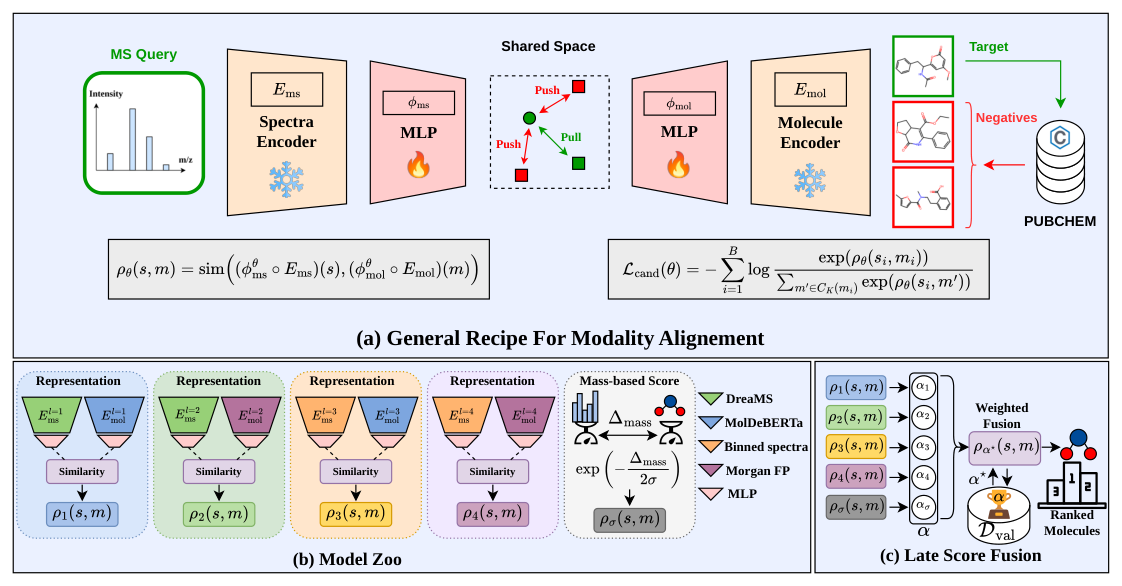
\includegraphics[width=\linewidth]{01-msalign-v2-recipe-model-zoo-late-fusion.png}
\caption{\lab{published}. \textbf{The MSAlign recipe}: frozen encoders joined by small trained networks, a ``model zoo''
of representation pairs plus a Gaussian mass scorer, and late fusion calibrated on validation data. Of the
representation pairs in panel (b), only DreaMS + Morgan fingerprint was retrained here; the MolDeBERTa pairs and the
fused model are published numbers only. Figure~1 from Krzakala et al., arXiv:2605.19752v2
(2026)~\citep{krzakala2026msalignv2}, CC~BY~4.0 (\url{https://creativecommons.org/licenses/by/4.0/}); cropped, caption removed.}
\label{fig:msalign}
\end{figure}

\subsection{Published numbers and their limits}\label{sec:published}
MSAlign v2, posted on 25 September 2026, reports formula-free results on the MassSpecGym formula split as means
and standard deviations over three split seeds (Table~\ref{tab:published}). Three things limit what such a table
can tell a reader. First, the paper's two versions disagree: v1 (19 May 2026) printed DeepSets at 22.2\% Recall@1 and
the DreaMS + fingerprint pair at 48.5\%, whereas v2 prints 4.7\% and 38.6\% for the same split; v1's headline 53.8\%
used ChemBERTa rather than MolDeBERTa, so it is a different model from v2's 47.5\%~\citep{krzakala2026msalignv1,
krzakala2026msalignv2}. Second, the strongest published rows were not run here: both v2 MSAlign models use
MolDeBERTa and have no released checkpoints (they ``will be released upon publication''~\citep{krzakala2026msalignv2}); MolDeBERTa is licensed
CC~BY-NC-ND~4.0~\citep{moldeberta_card}, and the candidate embedding cache would take about 20\,GB. JESTR, and the
formula-informed FLARE and MVP, need a Linux CUDA stack. Third, an audit by MassSpecGym's authors and others found
``evaluation issues in at least 17 of 26 papers reporting MassSpecGym benchmark results in the first year of its
adoption'', and showed that filtering a mass-based pool to the true formula alone lifts a random ranker's Hit@1
(Recall@1) from 0.43\% to 12.98\%~\citep{liu2026wild}. A published Recall@k describes one pool construction, one
split and one tie rule.

\begin{table}[tbp]
\centering
\footnotesize
\caption{\lab{published}. \textbf{MSAlign v2 formula-free results} (Tables~3 and~4 of~\citep{krzakala2026msalignv2}),
MassSpecGym formula split, Recall@k in \%, mean $\pm$ SD over three split seeds, official pools of up to 256 candidates
including repeated structures. The paper says only that a fixed tie-breaking rule was used; the released code counts
ties against the target~\citep{msalign_readme}. The standalone (47.5) and fused (58.2) MSAlign rows are different
models. Formula-known methods are omitted because they receive the true formula. Transcribed from the original
article; not re-extracted from the paper.}
\label{tab:published}
\begin{tabular}{@{}l r r r@{}}
\toprule
Method (MSAlign v2, published) & R@1 & R@5 & R@20 \\
\midrule
DeepSet (Fourier features, 50 epochs) & 4.7 $\pm$ 0.6 & 13.0 $\pm$ 1.3 & 27.5 $\pm$ 2.0 \\
JESTR & 13.9 $\pm$ 0.5 & 32.5 $\pm$ 0.8 & 57.0 $\pm$ 0.7 \\
Emb-Cos & 42.7 $\pm$ 3.0 & 65.2 $\pm$ 2.8 & 80.4 $\pm$ 1.6 \\
Binned + Fingerprint pair (Table 4) & 34.3 $\pm$ 1.3 & 56.2 $\pm$ 2.4 & 71.8 $\pm$ 1.3 \\
DreaMS + Fingerprint pair (Table 4) & 38.6 $\pm$ 2.8 & 60.4 $\pm$ 2.1 & 77.6 $\pm$ 0.8 \\
MSAlign, DreaMS + MolDeBERTa, standalone & 47.5 $\pm$ 3.4 & 71.3 $\pm$ 2.6 & 87.0 $\pm$ 1.1 \\
MSAlign fused (7 scores, 3 of them mass scores) & 58.2 $\pm$ 3.4 & 80.7 $\pm$ 3.0 & 92.8 $\pm$ 1.1 \\
\bottomrule
\end{tabular}
\end{table}

\subsection{Ties, pool size and declining}\label{sec:related}
Conventions differ across the literature. MSAlign's released code is strict~\citep{msalign_readme}, and Gupta et al.\
broke ties ``by random permutation''~\citep{gupta2026spurious}. Guo et al., writing about recommender systems, note
that such a gap ``follows mechanically from the tie block; it is not evidence that the score identified the relevant
item''~\citep{guo2026ties}. Small pools inflate weak methods' scores: Gin\'e et al.\ found that at 0.1\,ppm ``the
random-model baseline was substantially higher due to the smaller candidate pools''~\citep{gine2026}. Declining is not
a new idea either. COSMIC found the margin between hit and runner-up, and the number of candidates, to be ``highly
important features'' for confidence~\citep{hoffmann2022cosmic}, and MS2Query filtered unreliable matches with a score
threshold~\citep{dejonge2023ms2query}. J\"urgens et al.\ concluded that ``when the majority of predictions are
incorrect, any procedure with valid risk guarantees must abstain from making predictions for most instances'', and
named target-absent pools as ``an important open-world setting''~\citep{jurgens2026}; their default evaluation uses
formula-filtered pools that always contain the target. A conformal study found coverage falling below the nominal
level when calibration and test data came from different molecular clusters~\citep{rakhshaninejad2026}. Gupta et al.\ and
Gin\'e et al.\ varied candidate sets in other ways~\citep{gupta2026spurious,gine2026}. The specific
combination studied here (controlled target removal with validation-fitted thresholds and false-nomination rates for
formula-free alignment models, nested pool sizes from one mass window, and tie-rule effects) was not found in a dated
literature search on 4 October 2026.

%======================================================================
\section{Materials and methods}\label{sec:methods}

\subsection{Protocol}\label{sec:protocol}
The evaluation protocol was frozen on 4 October 2026 at 22:07:05Z (SHA-256 \m{aa2b30b5\ldots31b6}), before any
test-fold outcome of any method was computed or viewed; smoke runs used only training and validation rows. One
amendment, A1 (about 23:00\,UTC the same day, before any learned-model test score existed), added a descriptive
window-coverage measure (Section~\ref{sec:precursor}). The frozen original, the amended text and the freeze receipt
are archived in the results archive and copied to \m{protocol/historical/} in the repository. The freeze was the
original study's own record. It is not an approval under the repository's research harness, and it is not a protocol
for an independent reproduction.

\subsection{Data, split and populations}\label{sec:data}
The data are MassSpecGym as processed by the MSAlign authors (Zenodo 10.5281/zenodo.22830464,
CC~BY~4.0)~\citep{krzakala2026zenodo,bushuiev2024massspecgym}, split \m{formula\_seed1} (MSAlign v2 formula split, seed
1): training 210,825 spectra / 26,087 molecules; validation 9,631 / 1,428; test 10,648 / 1,421. All 10,648 test spectra
form the primary population, none excluded; every spectrum carries an [M+H]$^+$ or [M+Na]$^+$ adduct, charge $+1$ and a
precursor m/z. Spectra are not independent: 34.7\% of test rows match more than one MassSpecGym record with the same
structure, adduct, precursor and ten strongest peaks, so uncertainty is computed by resampling molecules. A
pre-declared secondary descriptive population, the official MassSpecGym \m{mces\_1} test fold (\MCESSpectra{}
spectra, \MCESMolecules{} molecules), was scored with the cheap baselines only (Appendix Table~\ref{tab:mces1}).

\subsection{Candidate pools}\label{sec:pools}
Pools were built once per target molecule and saved with hashes before scoring:
\begin{itemize}
\item \m{official\_raw}: the released 256-candidate mass list as distributed, duplicates counted with their
multiplicity (the published setting). Once stereochemistry is stripped, 85.4\% of the 28,936 official lists contain
at least one repeated structure (mean 6.9 repeats, maximum 121).
\item \m{official\_dedup} (\textbf{primary}): \m{official\_raw} with repeated 2D structures removed; median
\DedupMedian{} distinct structures.
\item \m{sub16}, \m{sub64}: the target plus 15 or 63 decoys drawn without replacement from \m{official\_dedup}, seeded
by the SHA-256 of the target SMILES.
\item \m{expanded1024}: \m{official\_dedup} plus decoys from the MassSpecGym 4M molecule set (a different database
snapshot) within 10\,ppm of the target's exact mass, excluding the target and existing members, capped at 1,024
structures (test median \ExpandedMedian, IQR 296--691; 5.1\% of the 2,849 validation and test targets reach the cap).
\item \m{absent}: \m{official\_dedup} with the target removed, a controlled stress test, not a measured rate of real
absence.
\end{itemize}
The target is in every pool except \m{absent}. Pool-size distributions are in Appendix Table~\ref{tab:poolsizes}.

\subsection{Methods compared}\label{sec:methods-list}
Every method receives the peak list (top 100 peaks as released), precursor m/z, adduct (hence charge), collision
energy where the released model uses it, and the candidate structures, and nothing else (Table~\ref{tab:methods}).
All learned models were newly trained with released code and settings, one seed (42) each, on one Apple M4 machine
with 16\,GB of memory: DeepSets with the released \m{model\_zoo} configuration (50 epochs, checkpoint by validation
loss); Emb-Cos with the released configuration (16,000 steps, checkpoint by validation Recall@1); and the MSAlign
alignment with the released \m{massspecgym\_formula} configuration and the molecule representation set to Morgan
(radius 2, 4,096 bits), 30,000 steps, checkpoint by validation Recall@1 (selected at step 3,296). The fusion weight
was chosen on validation Recall@5 over $w \in \{0, 0.05, \dots, 1\}$ (Appendix Table~\ref{tab:fusion}). For each
spectrum, the two component scores were z-scored using the mean and standard deviation over its \m{official\_dedup}
pool, target included. The same transformed scores were then used for every pool variant of that spectrum, including
\m{absent} (see Section~\ref{sec:abst-methods}). No reference
spectrum library search was run, because it would require library spectra for every candidate.

\begin{table}[tbp]
\centering
\footnotesize
\caption{\textbf{The formula-free methods run here.} All learned models were newly trained with released code and
settings, one seed (42) each. Fusion is exploratory and not a recommendation.}
\label{tab:methods}
\begin{tabularx}{\linewidth}{@{}>{\raggedright\arraybackslash}p{3.4cm} L L L@{}}
\toprule
Method & Spectrum input & Structure input & Score \\
\midrule
Random ordering & none & none & random order (expected value) \\
Precursor mass error & precursor m/z, adduct, charge & exact mass & smallest absolute ppm error first \\
DeepSets fingerprint predictor & peak list & Morgan fingerprint & cosine between predicted and candidate fingerprint \\
Emb-Cos & binned peaks & Morgan fingerprint & cosine in a learned shared space \\
DreaMS + Morgan (MSAlign code) & DreaMS embedding & Morgan fingerprint & cosine in a learned shared space \\
Alignment + mass fusion (exploratory) & DreaMS embedding and precursor & Morgan fingerprint and exact mass & weighted sum
of z-scored DreaMS + Morgan and mass-error scores; mass weight \FusionW{} chosen on validation Recall@5 \\
\bottomrule
\end{tabularx}
\end{table}

\subsection{Metrics and tie rules}\label{sec:metrics}
Recall@k is the share of test spectra whose true structure is among the first k ranked candidates; Recall@5 on
\m{official\_dedup} is primary, with Recall@1 and Recall@20 secondary. The primary tie rule is the expected value under
uniform random tie-breaking: for a target with $b$ decoys scoring strictly higher and $t$ decoys tied,
\begin{equation}
\mathrm{Recall@}k = \min\!\left(1, \max\!\left(0, \frac{k - b}{t + 1}\right)\right),
\end{equation}
so a target tied with three decoys counts as the average over the four possible orders. The released strict rule, in
which a tied decoy ranks ahead of the target, is reported alongside and used for comparison with published numbers.
Every test spectrum is in the denominator; a method that fails on a spectrum scores a miss, and there were no failures.
A later code review found that the archived abstention analysis did not implement this missing-spectrum rule: a
missing validation score made a fitted threshold undefined, and a missing test rank made nominated-recall estimates
undefined. The archived test-fold metrics record zero missing or failed spectra, and the defect is not known to have
affected any reported value.

\subsection{Uncertainty and pre-declared contrasts}\label{sec:stats}
Intervals are 95\% percentile intervals from 2,000 bootstrap resamples of target molecules (seed 20261004), resampling
all spectra of a chosen molecule together; paired contrasts use the same resampled molecules for both methods. Three
contrasts on Recall@5, \m{official\_dedup}, test, were declared before scoring: C1, DreaMS + Morgan minus mass error;
C2, DreaMS + Morgan minus Emb-Cos; C3, DeepSets minus mass error. Everything else is descriptive. With one split seed and
one training seed, intervals reflect which molecules were sampled, not variation between splits or training runs.

\subsection{Declining to nominate}\label{sec:abst-methods}
Confidence is the top-1 score in the pool (cosine for the learned models; minus the smallest absolute ppm error for mass
error); the margin between the top two scores is a secondary, exploratory confidence. Each validation spectrum is scored
twice, with \m{official\_dedup} (target present) and with \m{absent}. Two thresholds are fitted on validation only and then
frozen: one that keeps 90\% of target-present validation queries covered, and the lowest threshold at which at most 10\%
of target-removed validation queries are nominated. On test, ``covered'' is the share of target-present queries given a
shortlist and ``false'' the share of target-removed queries still given one.

\paragraph{Correction to exploratory fusion (6 October 2026).} Single-method scores do not depend on
which other candidates are in the pool. The original fusion implementation instead z-scored its components over
\m{official\_dedup} and reused those scores in other pools. Removing the target afterwards retained its influence
in the decoy scores. The corrected analysis standardises each component over the candidates actually present in
each evaluated pool; the raw pool uses multiplicity-weighted moments, and the absent pool excludes the target
before computing moments. The validation weight grid remains unchanged and selects $w=\FusionW$.
All fusion pool variants were rescored from the saved component scores. Thresholds were refitted using validation
only and applied once to test. Tables~\ref{tab:abstention} and~\ref{tab:abstention-all} report these corrected results.
The main official-deduplicated metrics, all nonfusion measurements and all reported paired contrasts were unchanged
within the predeclared absolute tolerance of $10^{-8}$ in their stored units. No models were retrained and no candidate
pools were regenerated. This retrospective correction is documented separately from the original frozen protocol.

\subsection{Reproduction check}\label{sec:repro-methods}
For the three trained models, the released evaluation (strict ties, \m{official\_raw}) on test was compared with the v2
paper's formula-split mean $\pm$ 2 SD. The scoring harness had to reproduce the trainer's own validation Recall@1 for the
selected checkpoint to 0.1 percentage points before any test scoring, and it reproduced each released evaluation exactly
on validation and test; for Emb-Cos and DeepSets the harness test values equal the released code's own end-of-training
evaluation (archived \m{released-result.json} receipts of runs T02 and T03) to 0.01 points.

\subsection{Execution and provenance}\label{sec:provenance}
All runs used one Apple M4 machine (10 cores, 16\,GB, macOS) without CUDA. Emb-Cos trained in 3.0 hours (16,000 steps) and
DreaMS + Morgan in \TrainHours{} hours (30,000 steps, selected checkpoint at step 3,296), so the difference in training time
partly reflects different step budgets. Run receipts were written by each run into its own immutable directory. The
tables use the corrected cached-score outputs where available and historical supplementary outputs otherwise.
Both sources are digest-checked (Appendix~\ref{app:provenance}). Training and model scoring were not repeated.

%======================================================================
\section{Results}\label{sec:results}

\subsection{Reproduction: at one seed only DreaMS + Morgan lands mostly inside the published band}\label{sec:repro}
Table~\ref{tab:repro} compares each retrained model, scored by the released rule, with the v2 paper's mean $\pm$ 2 SD.
DreaMS + Morgan sits just below the band on Recall@1 and inside it on Recall@5 and Recall@20; it peaked early
(validation Recall@1 0.376 after two epochs), and the released rule keeps that checkpoint. Emb-Cos fell below the band
on all three cut-offs. DeepSets landed far above v2 on all three; at Recall@5 and Recall@20 it sits closer to v1's
printed 36.1 and 50.9, and at Recall@1 (13.1) roughly midway between v2's 4.7 and v1's 22.2. With one split seed and one
training run, a miss shows where this run landed; it does not show that the paper is wrong.

\begin{table}[tbp]
\centering
\scriptsize
\setlength{\tabcolsep}{4pt}
\caption{\lab{reproduction}. \textbf{Released evaluation of the retrained models} on MassSpecGym formula split seed 1,
test fold, strict ties, official lists with duplicates kept, Recall@k in \%, one training seed (42) per model, against
the v2 paper's mean $\pm$ 2 SD. Source: archived \m{analysis/metrics.csv} (pool \m{official\_raw}, rule \m{strict}).}
\label{tab:repro}
\begin{tabularx}{\linewidth}{@{}>{\raggedright\arraybackslash}p{4.3cm} r r r >{\raggedright\arraybackslash}p{3.6cm} L@{}}
\toprule
Model (selected checkpoint) & R@1 & R@5 & R@20 & v2 mean $\pm$ 2 SD (R@1 / R@5 / R@20) & Verdict \\
\midrule
\inputtab{generated/tab_repro.tex}
\bottomrule
\end{tabularx}
\end{table}

\subsection{New measurement: both alignment models lead and were not separated}\label{sec:main}
Table~\ref{tab:main} and Figure~\ref{fig:recall} give the primary results. Either alignment model put the true structure
among the five confirmations for about six spectra in ten; mass error did so for fewer than one in seven. Every method
scored every spectrum. The pre-declared contrasts (Table~\ref{tab:contrasts}) show that C1 and C3 are well clear of zero:
DreaMS + Morgan beat mass error by 48.0 points of Recall@5 and DeepSets beat it by 18.0. No contrast was declared between
alignment and fingerprint prediction; the alignment models' intervals ([56.2, 66.3] and [58.4, 67.5]) do not overlap the
DeepSets interval [27.2, 35.5]. C2, at $-1.85$ points [$-5.19$, $+1.35$], includes zero: no detectable difference between
the two trained alignment models. That is not equivalence, and a modest gap in either direction is not ruled out. Nor is
C2 a test of spectral pretraining: the models differ in spectrum input, architecture, loss settings, training budget and
selected epoch, and each was trained once. The paper's controlled pair, DreaMS + fingerprint at 38.6\% against binned +
fingerprint at 34.3\% Recall@1, is published and was not reproduced here. The fusion with mass error reached 64.8\%
Recall@5, but it is exploratory, leans on recomputed precursor values (Section~\ref{sec:precursor}) and is not the
recommendation.

\begin{table}[tbp]
\centering
\footnotesize
\caption{\lab{new measurement}. \textbf{Primary results}: MassSpecGym formula split seed 1, 10,648 test spectra from
1,421 molecules, deduplicated official pools (median \DedupMedian{} structures), random-tie expectation, Recall@k in \%
with 95\% molecule-bootstrap intervals (2,000 resamples). Random ordering is the mean of 100 random orderings (equal to the analytic
expectation at printed precision), shown without an interval. Source: corrected \m{analysis/metrics.csv} and historical \m{analysis/random-repeats.json}.}
\label{tab:main}
\begin{tabular}{@{}l l l l@{}}
\toprule
Method & R@1 [95\% CI] & R@5 [95\% CI] & R@20 [95\% CI] \\
\midrule
\inputtab{generated/tab_main.tex}
\bottomrule
\end{tabular}
\end{table}

\begin{table}[tbp]
\centering
\footnotesize
\caption{\lab{new measurement}. \textbf{Pre-declared contrasts} (Recall@5, deduplicated official pools, test fold):
paired differences in percentage points on the same bootstrap resamples of molecules. The secondary contrasts at other
cut-offs, pools and rules are descriptive (Appendix Table~\ref{tab:contrasts-all}).}
\label{tab:contrasts}
\begin{tabular}{@{}l l@{}}
\toprule
Pre-declared contrast (Recall@5) & Difference, points [95\% CI] \\
\midrule
\inputtab{generated/tab_contrasts.tex}
\bottomrule
\end{tabular}
\end{table}

\begin{figure}[tbp]
\centering
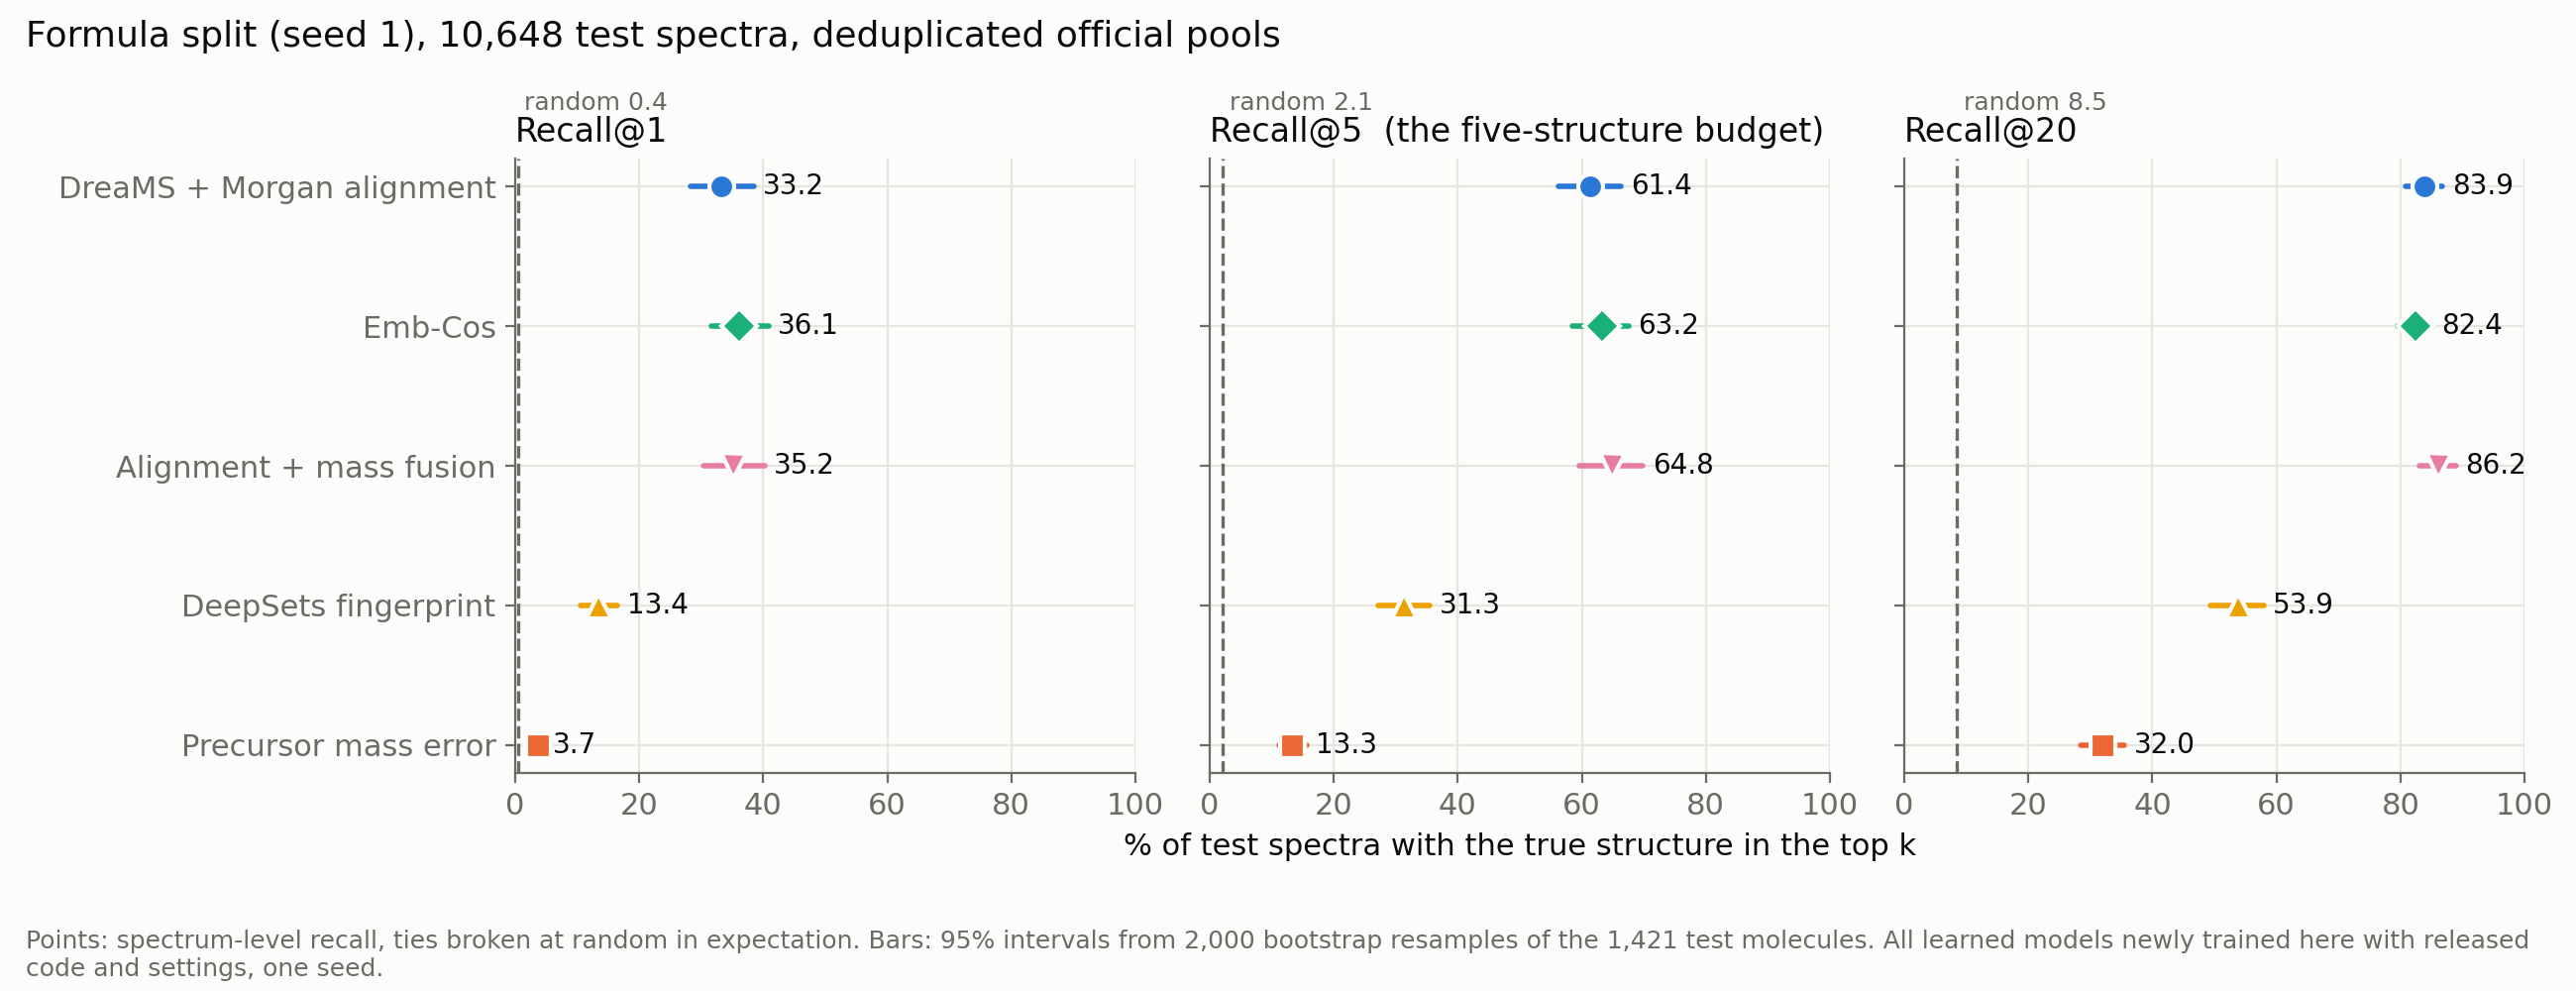
\includegraphics[width=\linewidth]{01-recall-by-method.png}
\caption{\lab{new measurement}. \textbf{Recall@1, @5 and @20 by method} on MassSpecGym formula split seed 1 (10,648 test
spectra, deduplicated official pools), ties broken at random in expectation. Bars are 95\% intervals from 2,000 bootstrap
resamples of the 1,421 test molecules; dashed lines are the random expectation. Higher is better. Original figure
\m{article/assets/01-recall-by-method.png}, drawn by the companion's \m{make\_charts.py} from the archived analysis.}
\label{fig:recall}
\end{figure}

\subsection{More candidates mean fewer hits for every method}\label{sec:poolsize}
The pool-size stress test kept the target in every pool (Figure~\ref{fig:pools}; Appendix Table~\ref{tab:pools}).
DreaMS + Morgan Recall@5 fell from 94.5\% at 16 structures to 81.4\% at 64, 61.4\% at \DedupMedian{} and 41.3\% at
\ExpandedMedian, and its Recall@1 from 69.2\% to 19.1\%. Random ordering fell from 31.2\% to 1.3\%. The order of method
families held at every size: alignment models (with or without fusion), then DeepSets, mass error and random ordering.
Within the top family it did not: DreaMS + Morgan led Emb-Cos at 16 structures (94.5\% against 93.8\%) and trailed at
\ExpandedMedian{} (41.3\% against 45.9\%), where corrected fusion (\FusionExpandedRecall{}\%) also fell below Emb-Cos. The expanded-pool paired
difference, $-4.56$ points [$-7.95$, $-1.19$], was not pre-declared and uses decoys drawn differently from the official
ones, so it is a reason to test both models at one's own list size, not a ranking. An expected Recall@5 should be quoted
with its list size.

\begin{figure}[tbp]
\centering
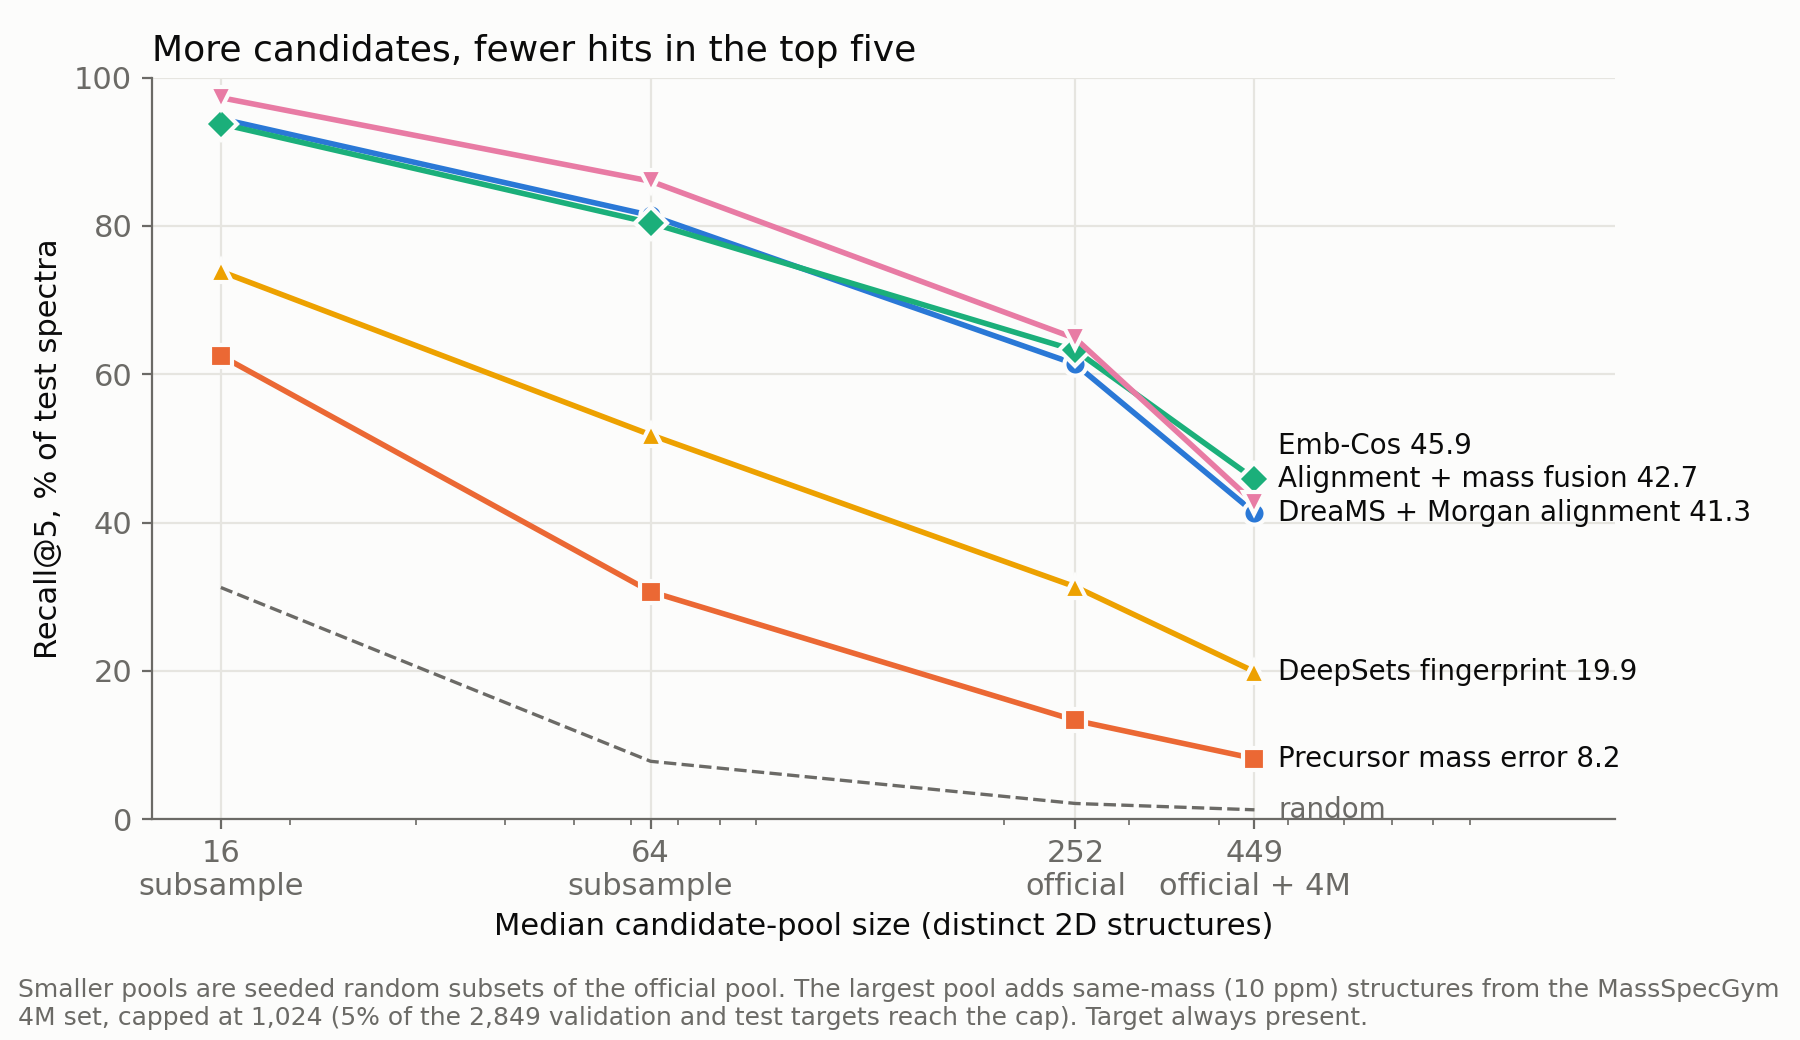
\includegraphics[width=0.85\linewidth]{02-pool-size-stress.png}
\caption{\lab{new measurement} (stress test). \textbf{Recall@5 against median pool size}, random-tie expectation, target
always present, 10,648 test spectra. The 16 and 64 pools are seeded subsets of the official pool; the \ExpandedMedian{}
pool adds same-mass structures from the MassSpecGym 4M set, a different database snapshot. Pool size is on a log scale.
Higher is better. Figure regenerated from corrected metrics; fusion uses each pool for normalisation.}
\label{fig:pools}
\end{figure}

\subsection{Scoring conventions move the cheap baseline most}\label{sec:rules}
Figure~\ref{fig:rules} and Table~\ref{tab:rules} apply counting conventions for ties and duplicates to identical scores.
Mass error doubled, from 6.3\% Recall@5 under the strict rule with duplicates kept to 13.3\% under the primary rule, and
its Recall@1 rose from 0.8\% to 3.7\%. The learned models moved by a few points: DreaMS + Morgan from 56.8\% to 61.4\%. Mass
error is hit hardest because every isomer of the target ties with it, and the strict rule counts all of them ahead of the
target. MSAlign v2's single Gaussian mass scorers reach only 0.6--0.8\% Recall@1 on their own~\citep{krzakala2026msalignv2},
which is consistent with strict counting on isomer-rich pools; that link is an inference. The rule should be stated next
to any reported number.

\begin{table}[tbp]
\centering
\footnotesize
\caption{\lab{new measurement}. \textbf{Recall@5 / Recall@1 (\%) under four counting conventions} applied to the same test
component scores. Fusion normalisation accounts for candidate multiplicity in raw pools. The first column uses the released
evaluation rule; the last is this study's primary rule. Source: corrected \m{analysis/metrics.csv}.}
\label{tab:rules}
\begin{tabular}{@{}l r r r r@{}}
\toprule
 & Strict, & Strict, & Random-tie, & Random-tie, \\
Method & duplicates kept & duplicates removed & duplicates kept & duplicates removed \\
\midrule
\inputtab{generated/tab_rules.tex}
\bottomrule
\end{tabular}
\end{table}

\begin{figure}[tbp]
\centering
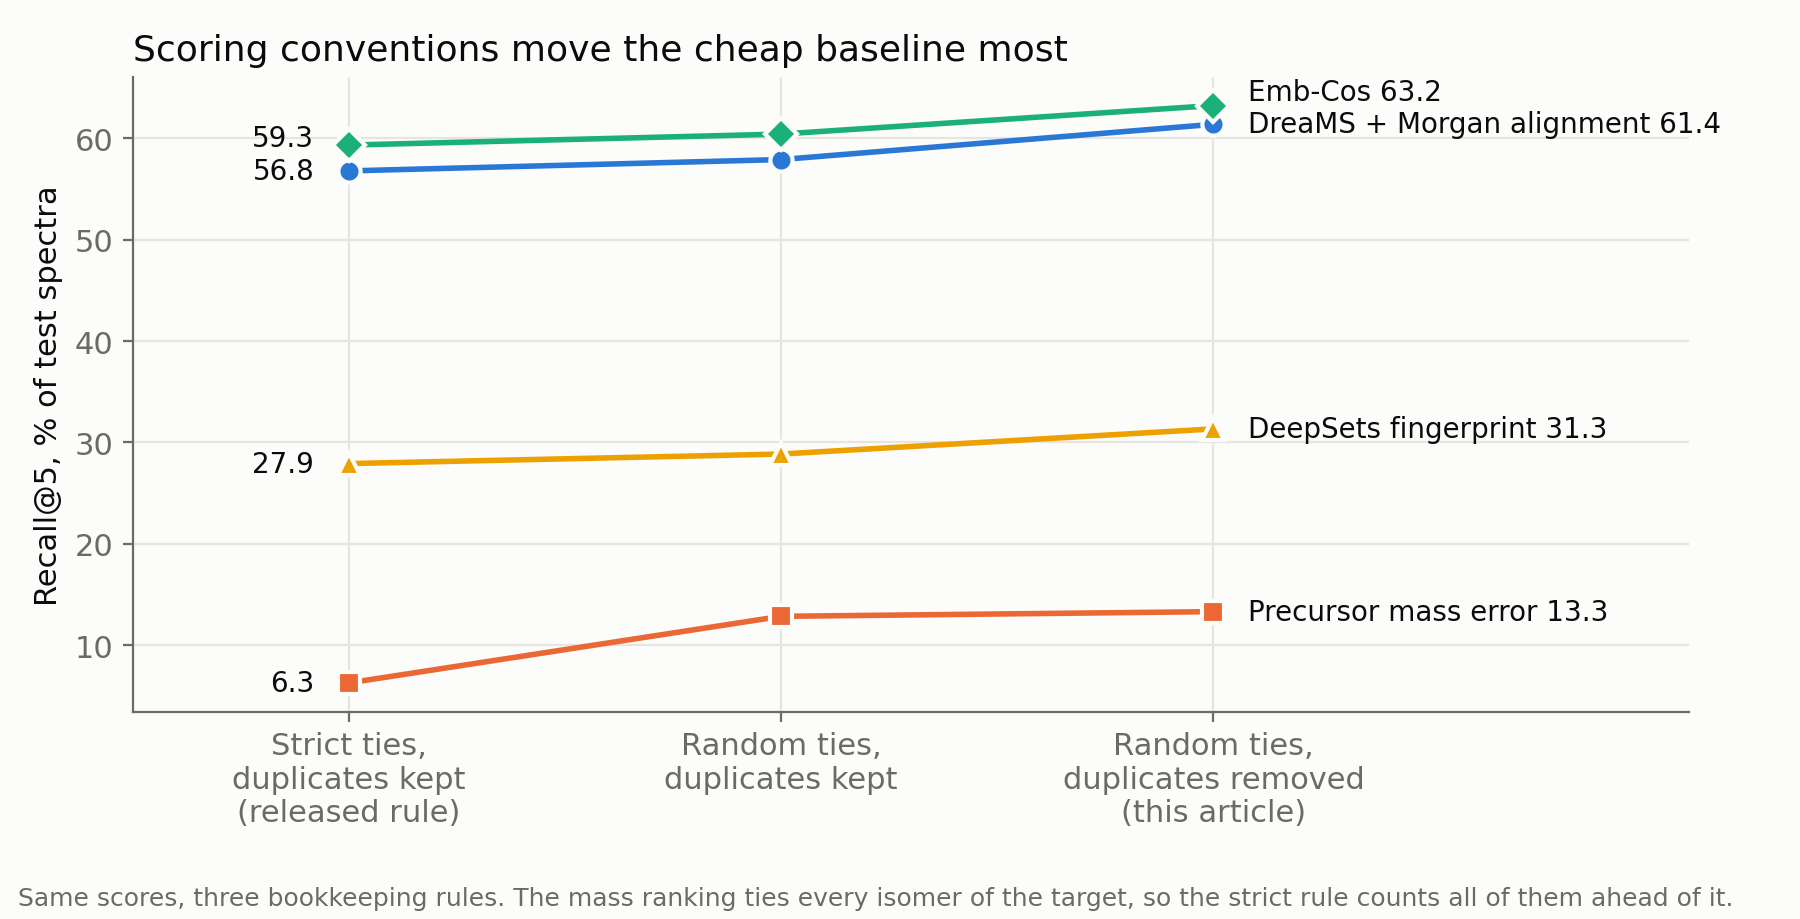
\includegraphics[width=0.85\linewidth]{03-tie-and-duplicate-rules.png}
\caption{\lab{new measurement}. \textbf{Recall@5 under three bookkeeping rules} applied to the same scores: the released
strict rule with duplicates kept, random-tie expectation with duplicates kept, and random-tie expectation with duplicates
removed (the primary rule). Original figure \m{article/assets/03-tie-and-duplicate-rules.png}.}
\label{fig:rules}
\end{figure}

\subsection{The top score is only a weak signal that the answer is missing}\label{sec:abstention}
Benchmark pools always contain the answer; a real search may not. Table~\ref{tab:abstention} and Figure~\ref{fig:decline}
report the target-removal stress test. Under the at-most-10\%-false rule, DreaMS + Morgan nominated for 21.3\% of
target-present test queries (68.4\% of those shortlists held the answer) and still nominated for 13.2\% of target-removed
ones; its validation-fitted threshold is \Threshold. The test false-nomination rates of the three single learned models
(13.2--15.7\%) all exceeded the 10\% validation target. Using the margin between the top two scores instead kept false
nominations under target but covered fewer queries: 13.8\% covered with 9.6\% false for DreaMS + Morgan, and 18.4\% with
9.8\% for Emb-Cos (Appendix Table~\ref{tab:abstention-all}). Mass error has no signal here: its coverage (12.2\%) equals its
false-nomination rate (12.1\%), because removing the target leaves its isomers with the same top score. The consequence is
a choice of failure mode. The 10\% threshold declines about four in five target-present queries; the 90\%-coverage
threshold nominates for 86.6\% of target-removed ones. In neither case is a cosine score a probability that the top
structure is right. Figure~\ref{fig:jurgens} reproduces the selective-prediction framing of J\"urgens et
al.~\citep{jurgens2026}.

\begin{table}[tbp]
\centering
\footnotesize
\setlength{\tabcolsep}{4pt}
\caption{\lab{new measurement} (stress test, artificial target removal). \textbf{Validation-fitted decline thresholds
applied once to test}, deduplicated official pools, confidence = top-1 score. ``Covered'' is the share of target-present
test queries given a shortlist; ``false'' the share of target-removed test queries still given one; 95\%
molecule-bootstrap intervals. Fusion uses corrected per-pool normalisation, with the target excluded before
normalising the absent pool. Source: corrected \m{analysis/abstention.csv}, indexed by
\m{evidence/corrected-analysis/current.json}.}
\label{tab:abstention}
\stackedci
\begin{tabular}{@{}l l l r l@{}}
\toprule
Method & Threshold rule & Covered & R@5 among & False nominations \\
 & (fitted on validation) & [95\% CI] & covered & [95\% CI] \\
\midrule
\inputtab{generated/tab_abstention.tex}
\bottomrule
\end{tabular}
\end{table}

\begin{figure}[tbp]
\centering
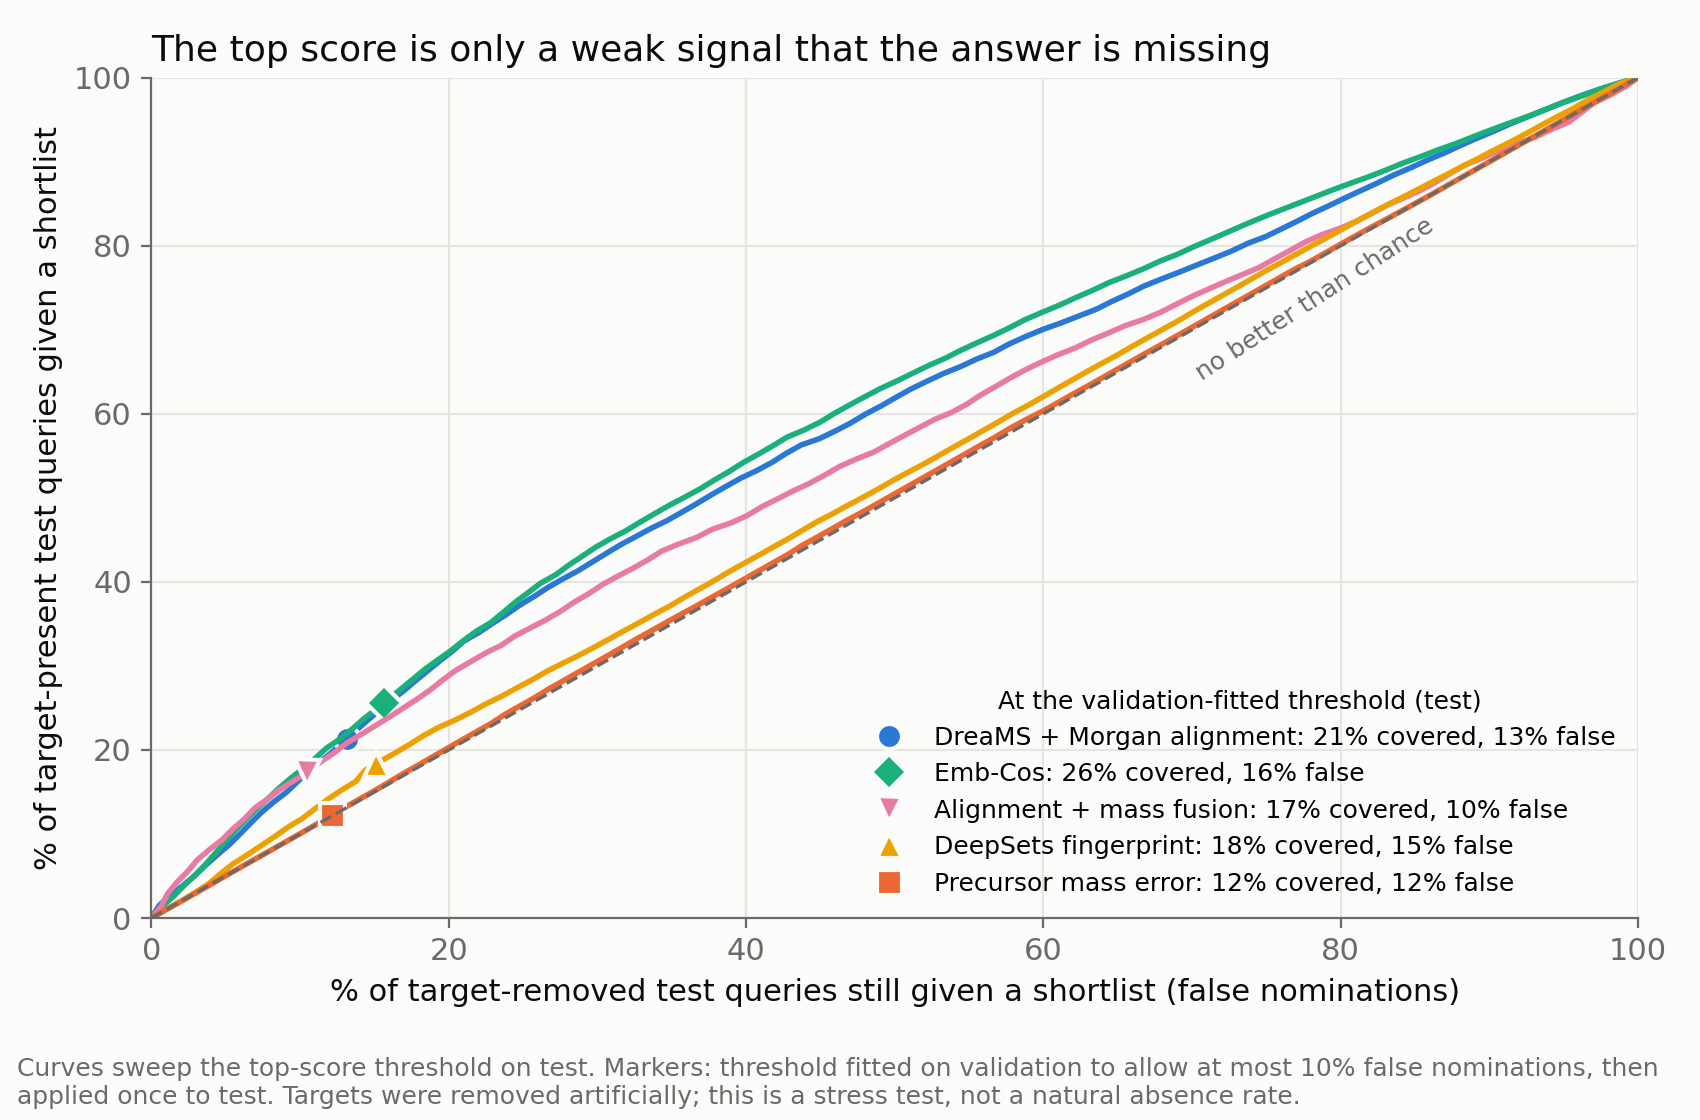
\includegraphics[width=0.78\linewidth]{04-decline-to-nominate.png}
\caption{\lab{new measurement} (stress test, artificial target removal). \textbf{Coverage of target-present queries against
false nominations on target-removed queries}, sweeping the top-score threshold on test; markers show the threshold fitted on
validation for at most 10\% false nominations. The diagonal is no better than chance. Legend values are rounded to whole
percentages; Table~\ref{tab:abstention} gives one decimal. Regenerated from corrected curves and thresholds.}
\label{fig:decline}
\end{figure}

\begin{figure}[tbp]
\centering
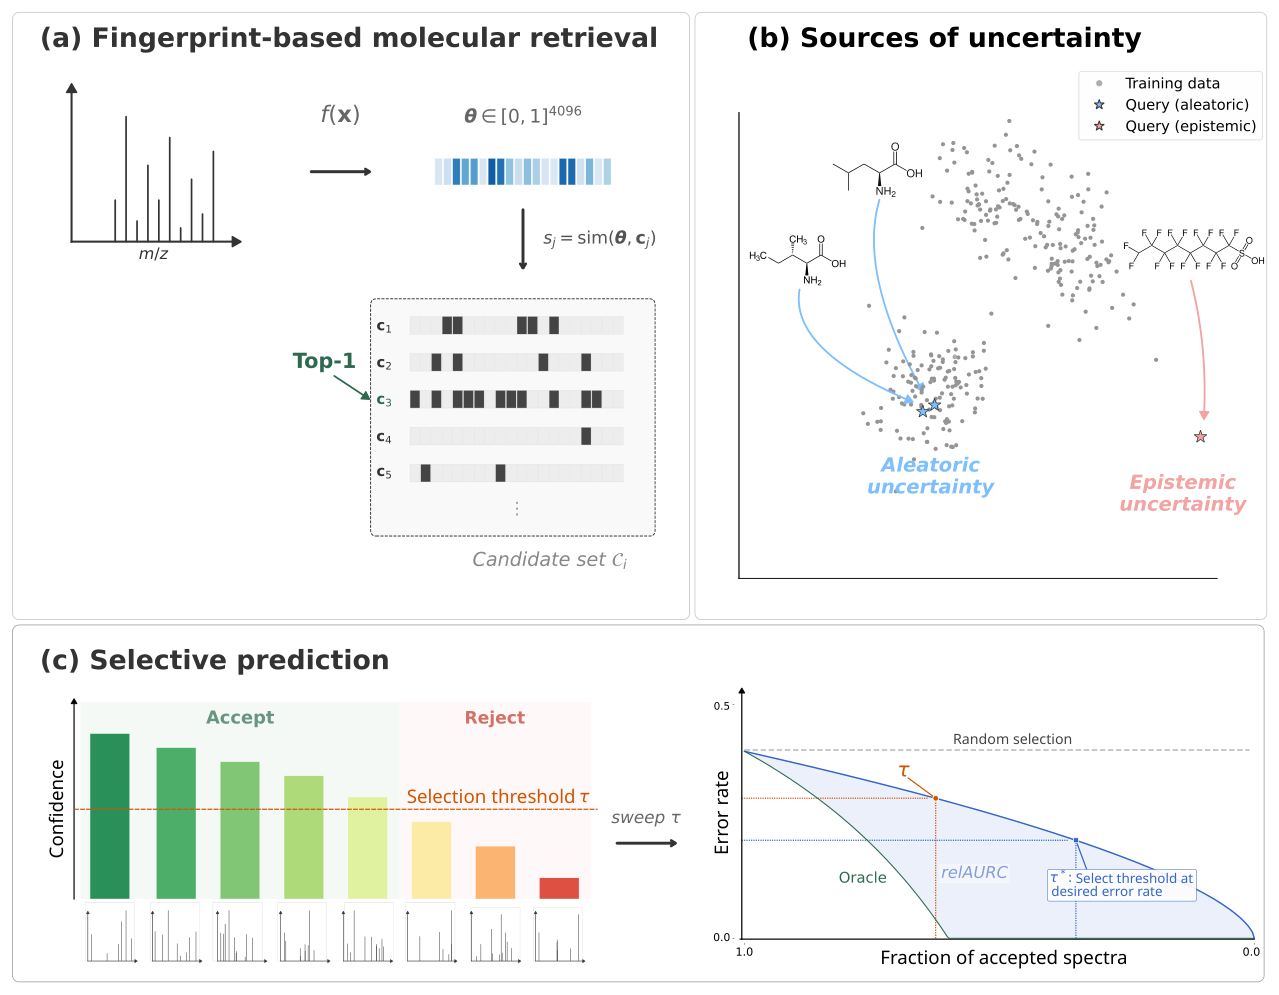
\includegraphics[width=0.72\linewidth]{13-jurgens-selective-prediction-overview.png}
\caption{\lab{published}. \textbf{Selective prediction as framed by J\"urgens et al.}: retrieval with a top-1 pick, sources of
uncertainty, and accepting or rejecting by a confidence threshold traced as a risk-coverage curve. Their default evaluation
uses formula-filtered pools that always contain the target, unlike the target-removal test here. Fig.~1 from J\"urgens et
al., arXiv:2603.10950v2 (2026)~\citep{jurgens2026}, CC~BY~4.0 (\url{https://creativecommons.org/licenses/by/4.0/}); cropped, caption removed.}
\label{fig:jurgens}
\end{figure}

\subsection{Check the precursor value before trusting any ranking}\label{sec:precursor}
In the training fold (n = 210,825), \TrainPrecursorWithin\% of spectra sit within 0.01\,ppm of the annotated structure's
theoretical mass (Figure~\ref{fig:precursor}; Appendix Table~\ref{tab:precursor}). Errors below 0.01\,ppm are far tighter
than the high (under 5\,ppm) or very high (under 1\,ppm) mass accuracy that Kind and Fiehn describe~\citep{kind2006}; they
suggest values recomputed from the annotation, as library curation can do: Spectraverse documents that ``parent masses were
recalculated from SMILES''~\citep{gupta2026spectraverse}. At the other end (amendment A1, exploratory), 6.94\% of test spectra
lie more than 10\,ppm from the annotated structure and 16.1\% more than 5\,ppm (validation 5.43\% and 9.2\%; \m{mces\_1} test
4.18\% and 15.4\%). These spectra keep their answer only because the benchmark pools are centred on the annotated
structure's mass; a real search centred on the measured precursor would lose it before any ranking, so for these spectra the
benchmark overstates what a real search would recover.

A post hoc split of the test fold by precursor error (Table~\ref{tab:strata}) shows where the mass baseline gets its strength:
31.6\% Recall@5 on recomputed-looking precursors and 9.2\% on the 0.01--10\,ppm group, which looks more like measured data.
The 21\% of test spectra in the first group supply about half of all its hits. Fusion added 8.4 points over DreaMS + Morgan
on recomputed precursors and 2.4 points on the 0.01--10\,ppm group, so much of its benefit comes from precursor values that
real measurements would not provide, which is why fusion stays exploratory. Mass is still worth using as a filter, because
it defines the pool; it should not be the ranker.

\begin{figure}[tbp]
\centering
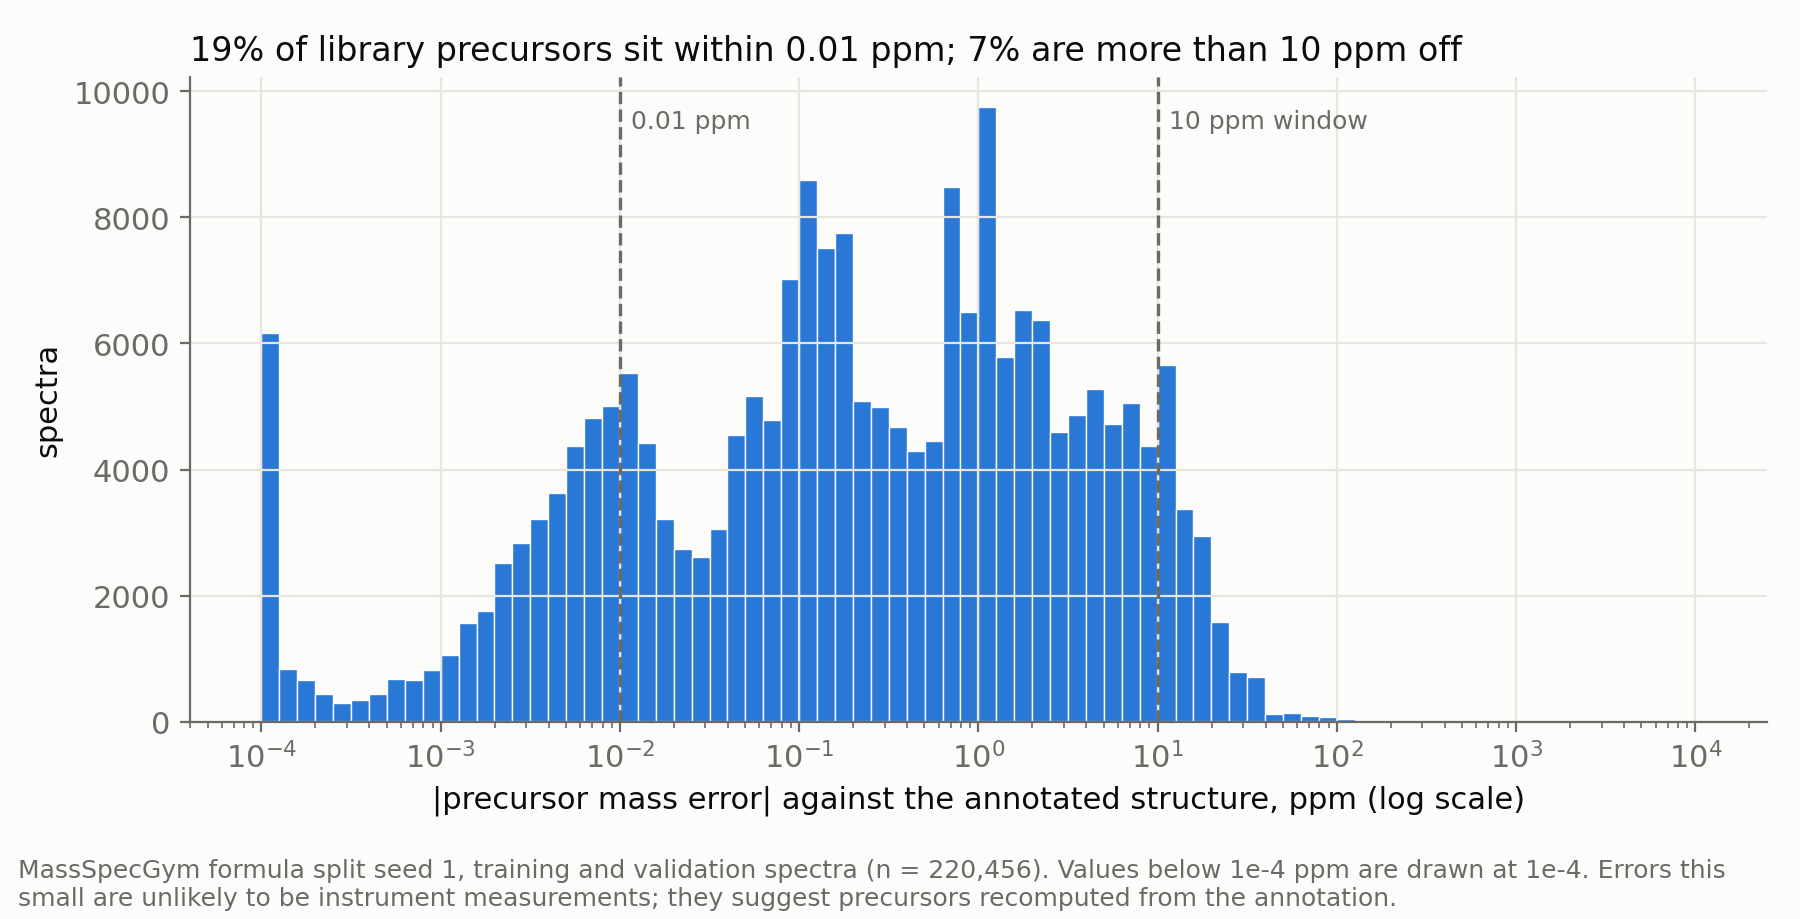
\includegraphics[width=0.85\linewidth]{05-precursor-mass-error.png}
\caption{\lab{new measurement} (data audit). \textbf{Absolute precursor mass error against the annotated structure} for
training and validation spectra (n = 220,456): 19.1\% within 0.01\,ppm, 7.07\% more than 10\,ppm away, median 0.211\,ppm. The
chart title rounds these to 19\% and 7\%. Values below $10^{-4}$\,ppm are drawn at $10^{-4}$. Original figure
\m{article/assets/05-precursor-mass-error.png}; per-fold summaries are in Appendix Table~\ref{tab:precursor}.}
\label{fig:precursor}
\end{figure}

\begin{table}[tbp]
\centering
\scriptsize
\setlength{\tabcolsep}{3pt}
\caption{\lab{post hoc}, descriptive. \textbf{Recall@5 (\%) by precursor-error stratum}, test fold, deduplicated official
pools, random-tie expectation, with 95\% molecule-bootstrap intervals. Source: archived \m{analysis/strata-post-hoc.csv}.}
\label{tab:strata}
\stackedci
\begin{tabular}{@{}l r l l l l l@{}}
\toprule
Stratum (post hoc) & Spectra / & Mass & DeepSets & DreaMS + & Emb-Cos & Fusion \\
 & molecules & error & & Morgan & & \\
\midrule
\inputtab{generated/tab_strata_precursor.tex}
\bottomrule
\end{tabular}
\end{table}

\subsection{The companion tool on the declared demonstration spectra}\label{sec:demo}
\paragraph{Inputs and outputs.} Spectra go in an MGF file with \m{PEPMASS}, \m{CHARGE} and \m{ADDUCT} in every block
(\m{COLLISION\_ENERGY} optional); candidates go in a CSV with \m{id} and \m{smiles} columns, frozen before any scores are
looked at. Supported adducts are [M+H]$^+$, [M+Na]$^+$, [M+NH$_4$]$^+$, [M+K]$^+$ and [M$-$H]$^-$; the trained model saw only the
first two, and other adducts run with a warning. Without \m{--model}, candidates are ranked by mass error alone and the run
never declines on score. With the model, the tool declines when the top score is below the value in
\m{models/thresholds.json}: \Threshold, the lowest value that nominated at most 10\% of target-removed validation queries. The
ranked CSV, still written after a decline, carries the score, \m{ppm\_error}, a decision column and tie flags
(\m{tied\_with\_previous}), and a provenance file is written alongside it that records the ppm window used.

\paragraph{Demonstration.} The companion tool follows the path in Figure~\ref{fig:path}: check metadata, check the ppm window, rank, compare the top
score with the validation-fitted threshold, then nominate five or decline. Mass-only runs skip the threshold step and never
decline on score. Its executed notebook ran the tool on two MassSpecGym test spectra chosen by a fixed rule before their
scores were viewed (the first [M+H]$^+$ and the first [M+Na]$^+$), and ran the [M+H]$^+$ spectrum again with its true
structure removed from the candidate file (verbatim outputs in Appendix~\ref{app:demo}). In the mass-only run on
MassSpecGymID0226249 ([M+H]$^+$, Orbitrap, 254 candidates), the annotated structure is one of 30 candidates tied at the same
mass, so the five nominated are an arbitrary cut. The model ranks it first yet declines, because its top score, 0.019, is
below the 0.599 threshold; with the structure removed it declines too. The [M+Na]$^+$ spectrum MassSpecGymID0395778 (QTOF)
fails before ranking: its recorded precursor, 826.4, is 117\,ppm below the ion implied by the annotated structure, so no
candidate lies within 10 or 50\,ppm; only the 200\,ppm window readmits 227 of the file's 229 candidates, and the model then
declines. Two deliberately invalid blocks were refused (missing adduct; charge inconsistent with the adduct). The DreaMS
weights reproduced the released embeddings (minimum cosine \VCosMin{} over \VSpectra{} spectra), and the exported model
matched the benchmark harness on the demo spectrum to within $2.2\times10^{-4}$, with the same rank. These outputs come from
the archived CLI. The revised CLI preserves isotope labels when removing stereochemistry, refuses unreadable metadata
per spectrum, discards invalid peaks and refuses spectra with no usable peaks or non-finite ranking scores
(\m{companion/README.md}). Missing collision energy remains represented by NaN; infinity is refused. The shared
chemistry helper also preserves isotope labels in future benchmark pool generation. Archived pools and results remain
unchanged. None of the demonstration inputs is isotope-labelled.

\begin{figure}[p]
\centering
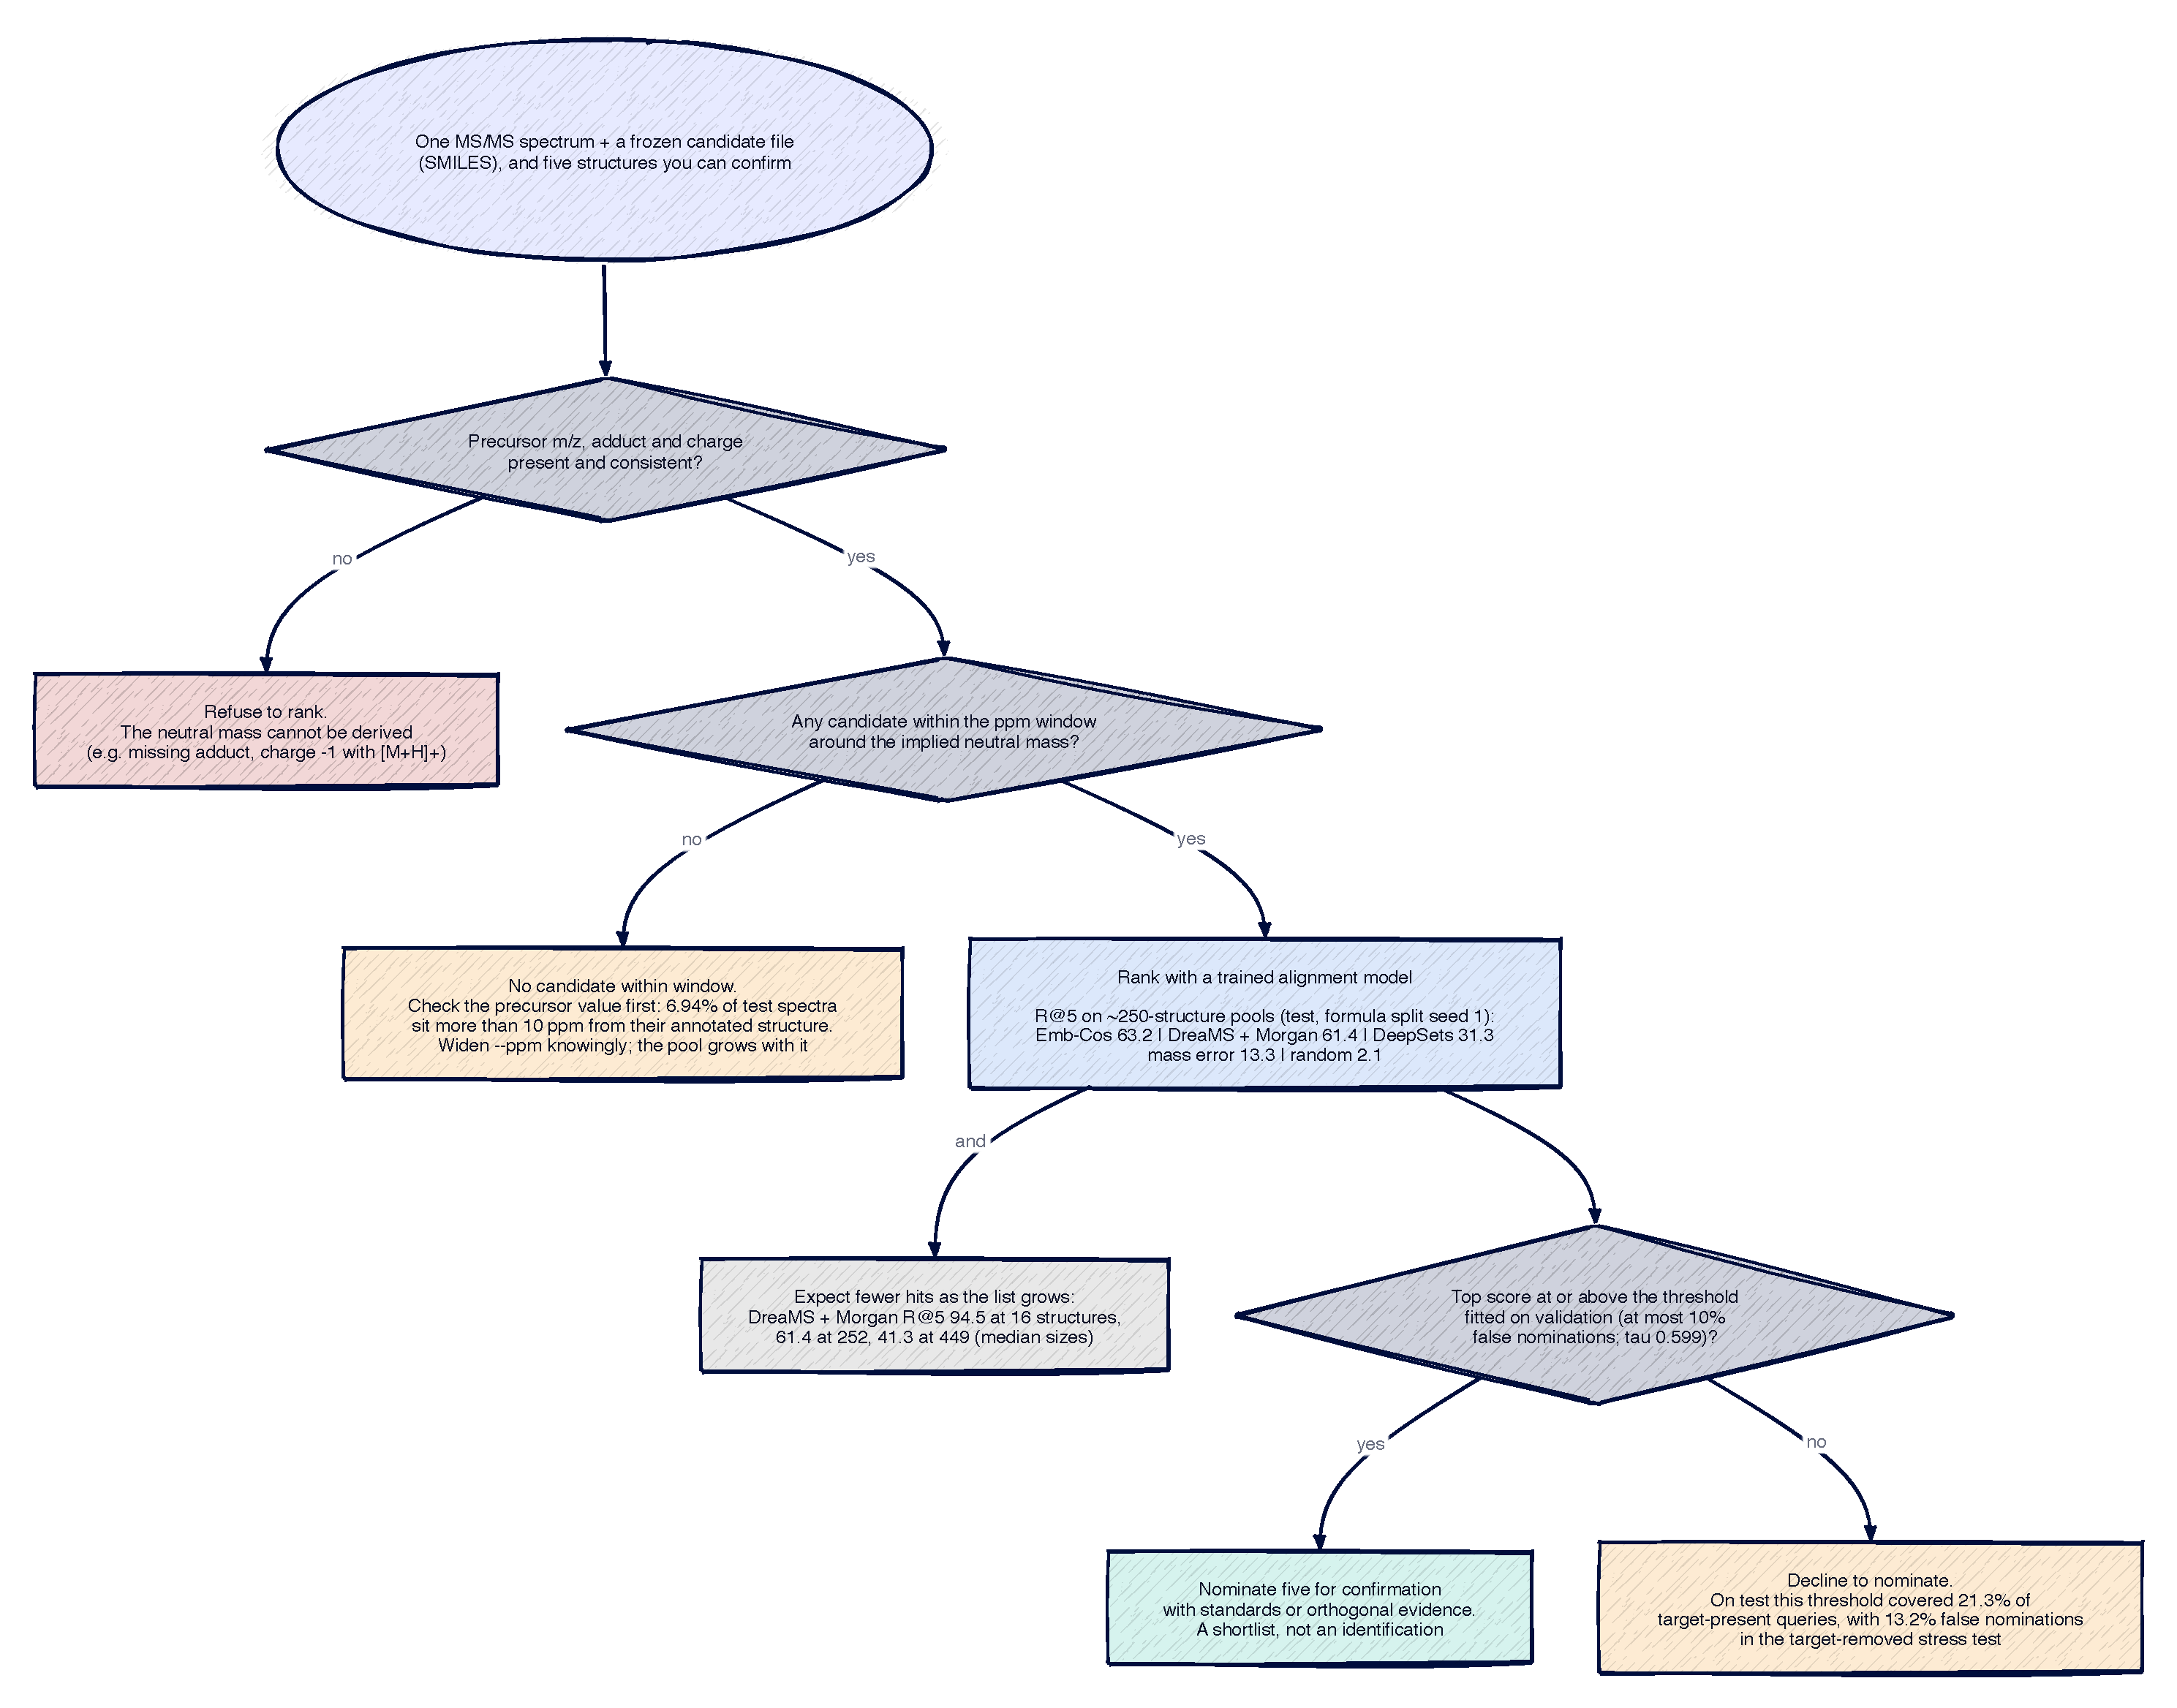
\includegraphics[angle=90,width=\linewidth,height=0.82\textheight,keepaspectratio]{01-decision-path.pdf}
\caption{\textbf{The decision path the companion tool follows for one spectrum}, with the benchmark numbers that bear on each
step (\lab{new measurement} and stress-test figures from Tables~\ref{tab:main} and~\ref{tab:abstention}, the pool-size stress
test and the precursor audit). Mass-only runs skip the threshold step and never decline on score. Converted from the original
\m{article/assets/01-decision-path.svg} (D2 source \m{01-decision-path.d2}).}
\label{fig:path}
\end{figure}

\subsection{Reproduction status}\label{sec:repro-status}
\noindent\fbox{\begin{minipage}{\dimexpr\linewidth-2\fboxsep-2\fboxrule\relax}\small
\textbf{Cached-score correction; independent training reproduction pending.} The correction reuses the original
candidate pools, saved component scores and nonfusion ranks. It recalculates fusion and refits its thresholds, preserving
all primary comparisons. Its execution and numerical checks are recorded separately in
\m{evidence/corrected-analysis/}. The reproduction reported in Section~\ref{sec:repro} is the original study's own
re-run of released code. Neither that comparison nor rerunning the cached correction constitutes independent retraining.
\end{minipage}}

%======================================================================
\section{Discussion}\label{sec:discussion}

\subsection{What to do in each situation}\label{sec:guidance}
If five candidate structures can be confirmed, a learned alignment model is the clear first choice for picking them on this
benchmark. The two alignment models showed no detectable difference; DreaMS + Morgan is the choice for users of the companion
tool as shipped (it is the bundled model), and the cheaper Emb-Cos recipe is reasonable for those training their own model,
who will need to score with it and fit its own decline threshold. More specifically:
\begin{itemize}
\item \textbf{Before ranking, check the precursor.} Compute the ppm error between the recorded precursor and the
best-supported candidate masses, and look at how many decimals the precursor carries. A value recorded to one decimal place,
like the 826.4 above, is too coarse for a 10\,ppm window at that mass. Recheck the raw file, adduct and charge first.
\item \textbf{If no candidate lies within the window,} recheck the precursor rather than widening the window. In a frozen file
a wider window only readmits that file's candidates; against a real database it admits far more structures, recall falls as
the pool grows (Figure~\ref{fig:pools}), and the shipped threshold was fitted on pools of about 250 mass-matched candidates.
Report the window beside any shortlist.
\item \textbf{After a decline,} the ranked list is still written, so a laboratory that prefers to inspect every list can ignore
the decision. Treat a decline as triage, not as evidence of absence, since most target-present queries are declined too. With
labelled spectra from one's own instrument and candidate source, refit the threshold on them~\citep{rakhshaninejad2026}.
\item \textbf{With mass-only ranking,} expect a shortlist every time; when a tie straddles the shortlist boundary, rank with an
alignment model rather than confirm an arbitrary five.
\item \textbf{Quote the list size} next to any expected hit rate, and if a list is much longer than \DedupMedian{} structures,
expect less than the official-pool numbers.
\end{itemize}

\subsection{What would change these conclusions}\label{sec:change}
Three results would change this advice: further seeds that separate Emb-Cos from DreaMS + Morgan; released MolDeBERTa
checkpoints showing whether the published standalone MSAlign's 71.3\% Recall@5 (v2, three-seed mean) holds under this
protocol; and a collapse towards chance on generated decoys that resemble library compounds, or under spectrum masking, which
would mean the alignment models lean on structure shortcuts.

%======================================================================
\section{Limitations}\label{sec:limitations}
\begin{itemize}
\item \textbf{One split seed, one training seed.} The intervals reflect which molecules were sampled, not variation between
splits or training runs.
\item \textbf{Untested methods.} MSAlign v2 standalone and fused (both MolDeBERTa), JESTR, FLARE, MVP and reference-spectrum
library search.
\item \textbf{Untested data.} No other split seeds, MCES-split training, Spectraverse, NPLIB1, instrument-held-out evaluation,
real target absence, negative-mode spectra or adducts beyond [M+H]$^+$ and [M+Na]$^+$. The post hoc instrument strata
(pre-specified as descriptive; DreaMS + Morgan Recall@5 57.2\% [51.3, 63.1] on Orbitrap, 71.2\% [64.7, 76.8] on QTOF; Appendix
Table~\ref{tab:strata-instrument}) are confounded by which molecules each instrument measured.
\item \textbf{Possible encoder overlap.} The DreaMS checkpoint loaded by the MSAlign code was fine-tuned on a MoNA subset (about
25,000 spectra, 5,500 InChI connectivity blocks)~\citep{bushuiev2026dreams}, and MassSpecGym draws spectra partly from
MoNA~\citep{bushuiev2024massspecgym}. Overlap with the test molecules was not checked: an unmeasured possibility, not a
finding.
\item \textbf{Near-duplicate records.} 34.7\% of test rows match more than one MassSpecGym record with the same structure,
adduct, precursor and ten strongest peaks, so spectra are not independent; that is why the intervals resample molecules.
\item \textbf{Benchmark pools contain the answer.} Target removal is artificial, and pools centred on the annotated mass keep
answers that a search centred on the measured precursor would lose (Section~\ref{sec:precursor}).
\item \textbf{Shortcut controls.} The alignment models were not tested against generated decoys that resemble library
compounds~\citep{gupta2026spurious}, nor by ``masking all input MS/MS spectra with a constant value and confirming that
performance degrades accordingly''~\citep{liu2026wild}.
\item \textbf{Fusion correction has limited scope.} The historical target-removal values retained information
from the target during normalisation and are superseded here. Corrected fusion removes the target before normalisation
and recalibrates on validation. This remains an artificial target-removal stress test, not a deployment guarantee.
The cached-score correction does not test different training seeds or rebuild the candidate pools.
\item \textbf{Code defects found after the analysis.} A later review found defects in the companion CLI (isotope labels
dropped along with stereochemistry; unreadable metadata or non-finite values could crash a batch or yield a nomination),
in the training queue's exit status, in the paper validator's digest checks, and in the abstention analysis's handling of
missing spectra. The archived runs recorded no missing or failed spectra, and those complete-case single-method results were unchanged by reanalysis. The demonstration outputs in Section~\ref{sec:demo} come from the archived CLI.
\item \textbf{Exploratory and post hoc analyses.} Fusion, the margin confidence, the expanded-pool contrast, the precursor and
instrument strata and the window-coverage measure are exploratory or post hoc. Only C1--C3 were pre-declared contrasts; the instrument
strata and the \m{mces\_1} population were pre-declared as descriptive. None of the intervals is adjusted for multiplicity.
\item \textbf{No identification.} The MSI minimum for a level~1 identification of a known metabolite is ``a minimum of two
independent and orthogonal data relative to an authentic compound analyzed under identical experimental
conditions''~\citep{sumner2007msi}. The confidence scale of Schymanski et al.~\citep{schymanski2014} invites researchers to
define sublevels ``on a per-study basis where evidence supporting different proposed structures is clearly
presented''~\citep{charbonnet2022}. Every nominee should be confirmed against an authentic standard.
\end{itemize}

%======================================================================
\section{Data, code and licence availability}\label{sec:availability}
The study repository (\texttt{rewire-bio/msms-model-selection}) contains this manuscript and its build (\texttt{make
paper-imported}); the original article (\texttt{article/original.md} and the byte-identical
\texttt{article/published-original.md}, also embedded in this PDF as Supplement~S1); the maintained companion code (\texttt{companion/}); its historical snapshot
(\path{downloads/msms-shortlist-companion-code.tar.gz}, 0.18\,MB, without the later fixes); the trained DreaMS + Morgan model and threshold
(45\,MB, split for a 25\,MiB file limit; see below); and the historical results archive (\path{downloads/msms-shortlist-results.tar.gz}, about 7\,MB) with
original analysis outputs, per-spectrum predictions and run receipts. Corrected outputs and their checksums are indexed
by \m{evidence/corrected-analysis/current.json}. The 401.7\,MB of cached inputs used for correction are hash-identified
but not distributed in Git; repeating the correction requires those preserved files. The DreaMS TorchScript weights (468\,MB, MIT
licence~\citep{dreams_card}) are not bundled and are downloaded from Hugging Face \m{roman-bushuiev/DreaMS} at revision
\m{c81a62766b10}.

The model bundle consists of five files in \m{downloads/}:
\begin{itemize}\small
\item \m{msms-shortlist-dreams-morgan-model.tar.gz.part01}, \m{.part02} and \m{.part03};
\item \m{reassemble-model.sh} and \m{msms-shortlist-dreams-morgan-model.parts.sha256}.
\end{itemize}
Saving all five in one folder and running \m{sh reassemble-model.sh} checks each part, joins them in order, verifies the SHA-256
of the joined archive and extracts the model. The joined archive's SHA-256 is
\begin{center}\footnotesize\m{646bbe4fbb14bda60e3544d4a963c9319b6564663c9b0752cd5e92b879eeffc9}.\end{center} The companion code is
MIT-licensed, and \m{towers.py} adapts MSAlign inference code (MIT). Data and weights keep their own licences: MassSpecGym
(MIT), the MSAlign Zenodo bundle (CC~BY~4.0), DreaMS weights (MIT); MolDeBERTa (not used) is CC~BY-NC-ND~4.0. The two
reproduced literature figures are CC~BY~4.0 and are attributed in their captions.

%======================================================================
\section{AI assistance, review and disclosure}\label{sec:disclosure}
This manuscript was drafted by an AI model (Claude Opus, \texttt{claude-opus-5-5}) from the archived evidence. A draft was
reviewed by an independent AI reviewer instance of the same model (\texttt{evidence/paper-migration/review.md}, 18 findings),
and the author's disposition of every finding is in \texttt{evidence/paper-migration/review-disposition.md}; this version
incorporates those corrections. The original article does not state who ran the analyses or how it was reviewed, and this
manuscript makes no claim about either. Codex coordinated the 6 October cached-score correction and updated the manuscript,
with a separate Codex agent checking methods and numerical outputs. The owner authorised that correction.
No human scientific review of this manuscript has taken place.

%======================================================================
\bibliographystyle{unsrtnat}
\bibliography{references}

%======================================================================
\clearpage
\appendix
\section{Reproducing the historical run}\label{app:repro}
The commands below are those recorded in the original article and the companion README; they were executed for the original
article and were \emph{not} re-executed for this manuscript. \m{uv sync} uses \m{uv.lock} (torch 2.2.1, rdkit 2023.9.6, numpy
1.25.0, pandas 2.2.1).
\begin{lstlisting}
uv sync

# Mass-error ranking only (no model files needed)
uv run msms-shortlist --spectra examples/mh.mgf \
    --candidates examples/mh-candidates.csv --out out/mh-mass.csv

# Trained DreaMS + Morgan alignment model
uv run msms-shortlist --spectra examples/mh.mgf \
    --candidates examples/mh-candidates.csv \
    --model models/dreams_morgan_formula_seed1_fp16.pt \
    --dreams weights/DreaMS_embedding_model_torchscript.pt \
    --thresholds models/thresholds.json --out out/mh-model.csv
\end{lstlisting}
From a clean archive, \m{uv sync} took 1.5\,s with a warm cache, the first CLI run 35\,s including the package build, and a model
run 5.3\,s. The benchmark pipeline (MSAlign checkout at \m{c2ef425}, one storage patch, training, frozen pools, scoring, rank
statistics, fusion and analysis) is listed command by command in \m{companion/REPRODUCE.md}, with data hashes and run receipts.

\paragraph{Rebuilding this manuscript.} \m{make paper-imported} runs \m{scripts/build\_paper.py} with the system Python and local
TeX Live. It verifies the archive and member digests, formats the tables in \m{paper/generated/}, converts the original
decision-path SVG with \m{rsvg-convert}, and runs pdflatex, BibTeX and pdflatex twice. It performs no experiment, data download,
model inference or environment creation. The receipt is \m{evidence/paper-migration/build-receipt.json}.

\section{Recorded demonstration outputs}\label{app:demo}
Verbatim from the original article; each block is output from the run named above it, and lines without a query identifier were
printed by the notebook from the run's provenance file or ranked CSV.
\begin{lstlisting}[basicstyle=\ttfamily\scriptsize]
# Mass-only run, MassSpecGymID0226249 ([M+H]+, Orbitrap, 254 candidates)
MassSpecGymID0226249: nominate shortlist
tie at shortlist boundary: True | candidates sharing the 5th score: 30

# Model run, same spectrum
MassSpecGymID0226249: decline: top score below validation threshold
decision: decline: top score below validation threshold | top score: 0.0194 | threshold: 0.5994
rank of the annotated structure: 1

# Model run, true structure removed
MassSpecGymID0226249: decline: top score below validation threshold
decision with the true structure removed: decline: top score below validation threshold | top score: -0.0245

# [M+Na]+ model runs, MassSpecGymID0395778 (QTOF), --ppm 10, 50 and 200
MassSpecGymID0395778: no candidate within window (no structure within 10.0 ppm)
10 ppm: no candidate within window | candidates in window: 0
MassSpecGymID0395778: no candidate within window (no structure within 50.0 ppm)
50 ppm: no candidate within window | candidates in window: 0
MassSpecGymID0395778: decline: top score below validation threshold
200 ppm: decline: top score below validation threshold | candidates in window: 227

# Invalid-metadata run (mass-only)
no_adduct_example: refused (missing ADDUCT; the neutral mass cannot be derived)
wrong_charge_example: refused (charge -1 is inconsistent with adduct [M+H]+)
\end{lstlisting}
The archived consistency check between the CLI and the benchmark harness on the demonstration spectrum
(\m{receipts/X02-cli-demo-\ldots/consistency-check.txt}) reads, verbatim:
\lstinputlisting{generated/cli_consistency.txt}

\section{Supplementary tables}\label{app:supp}
Tables use corrected cached-score results where available; unaffected supplementary analyses remain historical.

\begin{table}[H]
\centering
\footnotesize
\caption{\lab{new measurement}, descriptive. \textbf{Candidate-pool sizes} per test spectrum (10,648 spectra), counting
distinct 2D structures; for \m{official, raw} the multiplicity-weighted list length is not summarised in the archive, so its
row equals the deduplicated one. Source: \m{pool-sizes.csv} in the archived \m{analysis/}.}
\label{tab:poolsizes}
\begin{tabular}{@{}l r r r r r r r@{}}
\toprule
Pool & Spectra & Mean & Min & 25\% & Median & 75\% & Max \\
\midrule
\inputtab{generated/tab_poolsizes.tex}
\bottomrule
\end{tabular}
\end{table}

\begin{table}[H]
\centering
\footnotesize
\caption{\lab{new measurement} (stress test). \textbf{Recall@5 and Recall@1 (\%) by pool}, random-tie expectation, target always
present; random ordering is the mean of 100 random orderings (equal to the analytic expectation at printed precision). Source: corrected \m{analysis/metrics.csv} and historical
\m{analysis/random-repeats.json}.}
\label{tab:pools}
\begin{tabular}{@{}l l r r r r@{}}
\toprule
 & & \multicolumn{4}{c}{Median pool size} \\
\cmidrule(l){3-6}
k & Method & 16 & 64 & \DedupMedian{} (official) & \ExpandedMedian{} (expanded) \\
\midrule
\inputtab{generated/tab_pools.tex}
\bottomrule
\end{tabular}
\end{table}

\begin{table}[H]
\centering
\scriptsize
\setlength{\tabcolsep}{3pt}
\caption{\lab{new measurement} (stress test; margin-confidence rows exploratory). \textbf{All decline-threshold results}: both confidences (top-1 score and the exploratory top-two margin) and both
rules, with the fitted threshold, its validation false-nomination rate (\%) and test coverage, Recall@5 among covered and false
nominations (\%, 95\% intervals). Fusion rows use corrected per-pool normalisation and validation-only recalibration;
the absent target is excluded before computing the component moments. Other methods are unchanged. Source:
corrected \m{analysis/abstention.csv}, indexed by \m{evidence/corrected-analysis/current.json}.}
\label{tab:abstention-all}
\stackedci
\begin{tabular}{@{}l l l r r l l l@{}}
\toprule
Method & Conf. & Rule & Threshold & Val. & Covered & R@5 among & False \\
 & & & & false & & covered & nominations \\
\midrule
\inputtab{generated/tab_abstention_all.tex}
\bottomrule
\end{tabular}
\end{table}

\begin{table}[H]
\centering
\scriptsize
\setlength{\tabcolsep}{3pt}
\caption{Descriptive. \textbf{Recall@5 (\%) by instrument stratum}, test fold, deduplicated official pools, 95\% intervals.
Pre-specified as descriptive in the frozen protocol (\S5) and labelled post hoc in the original article; 862 test spectra could
not be mapped. Confounded by which molecules each instrument measured. Source: archived \m{analysis/strata-post-hoc.csv}.}
\label{tab:strata-instrument}
\stackedci
\begin{tabular}{@{}l r l l l l l@{}}
\toprule
Instrument & Spectra / & Mass & DeepSets & DreaMS + & Emb-Cos & Fusion \\
 & molecules & error & & Morgan & & \\
\midrule
\inputtab{generated/tab_strata_instrument.tex}
\bottomrule
\end{tabular}
\end{table}

\begin{table}[H]
\centering
\footnotesize
\caption{Exploratory. \textbf{Fusion weight selection}: validation Recall@5 (\%) on deduplicated official pools for each mass weight $w$;
$w = \FusionW$ was chosen. Source: corrected \m{fusion-weight.json}; the complete validation grid is unchanged from the original.}
\label{tab:fusion}
\begin{tabular}{@{}r r r r@{}}
\toprule
$w$ & Val.\ R@5 & $w$ & Val.\ R@5 \\
\midrule
\inputtab{generated/tab_fusion.tex}
\bottomrule
\end{tabular}
\end{table}

\begin{table}[H]
\centering
\footnotesize
\caption{\lab{new measurement} (data audit). \textbf{Precursor mass error against the annotated structure}, percentage of
spectra below each threshold and median absolute error (ppm). Source: archived
\m{receipts/A02-precursor-error-audit-\ldots/summary.json}.}
\label{tab:precursor}
\begin{tabular}{@{}l r r r r r r r@{}}
\toprule
Fold & Spectra & $<$0.01 & $<$0.1 & $<$1 & $<$5 & $<$10 & Median \\
\midrule
\inputtab{generated/tab_precursor.tex}
\bottomrule
\end{tabular}
\end{table}

\begin{table}[tbp]
\centering
\scriptsize
\caption{\lab{new measurement}, descriptive. \textbf{Pre-declared secondary population}: the official MassSpecGym \m{mces\_1} test
fold (\MCESSpectra{} spectra, \MCESMolecules{} molecules), cheap baselines only, Recall@k (\%) with 95\% molecule-bootstrap
intervals; random ordering is the analytic expectation. Under the strict rule every candidate ties for random ordering, so it
scores 0 except where the pool is no larger than $k$ (pool 16 at $k = 20$). Median deduplicated pool size \MCESDedupMedian{}
(\m{sub64} minimum \MCESSubMin). These results were archived but not reported in the original article. They are not
comparable with Tables~\ref{tab:main} and~\ref{tab:pools}: the fold and molecules differ, and its share of recomputed-looking
precursors was not audited. Source: archived \m{analysis-mces1/metrics.csv}.}
\label{tab:mces1}
\begin{tabular}{@{}l l l r l@{}}
\toprule
Pool & Rule & Method & k & Recall [95\% CI] \\
\midrule
\inputtab{generated/tab_mces1.tex}
\bottomrule
\end{tabular}
\end{table}

\scriptsize
\setlength{\tabcolsep}{3pt}
\begin{longtable}{@{}l l l r l l@{}}
\caption{\normalsize\lab{new measurement}. \textbf{All archived paired contrasts} (percentage points, 95\% molecule-bootstrap
intervals). Only the three rows marked as primary were pre-declared; all others are descriptive. With 16 candidates every method
has Recall@20 = 100\%, so those contrasts are exactly zero. Source: archived \m{analysis/contrasts.csv}.}
\label{tab:contrasts-all}\\
\toprule
Contrast & Pool & Rule & k & Primary & Difference [95\% CI] \\
\midrule
\endfirsthead
\toprule
Contrast & Pool & Rule & k & Primary & Difference [95\% CI] \\
\midrule
\endhead
\bottomrule
\endfoot
\inputtab{generated/tab_contrasts_all.tex}
\end{longtable}
\normalsize

\section{Provenance, supplement and evidence mapping}\label{app:provenance}
\paragraph{Supplement S1 (original article).} The full original article, \emph{An MS/MS Shortlist Is Not an Identification:
Choosing a Formula-Free Ranker and Knowing When to Decline} (5 October 2026), is retained unchanged as
\m{article/published-original.md} (byte-identical to the published source) and is embedded in this PDF as the attachment
\m{S1-published-original.md}; \m{article/original.md} differs only in local links. Its fusion pool-variant and abstention results are superseded by the correction in this manuscript, and \m{content-coverage.md} in \m{evidence/paper-migration/} maps it section by section.

\paragraph{Evidence ledger.} \m{evidence/paper-migration/claims-ledger.json} links each substantive claim to a
historical or corrected artifact, a pointer inside it and its SHA-256. The original archive is digest-checked and its
published values are checked at printed precision before any corrected tables are rendered. A second pass reads the
corrected metrics, contrasts, abstention results and fusion grid from the separately hashed execution outputs.
The correction index and run receipt bind those inputs to their saved comparisons and provenance. Figures for pool-size
stress and abstention are regenerated from the same corrected tables. Unaffected supplementary analyses, training records,
random-order repeats and the secondary \m{mces\_1} population remain historical. Counts or timings available only in
article text or protocol notes remain labelled as such. Cached inputs were hashed at correction time; this does not
independently establish the authenticity of their original acquisition.

\paragraph{Citation note.} Literature claims were verified for the original article (citation status ``verified'') and were not
re-retrieved during migration. Table~\ref{tab:published} is transcribed from the original article.

\end{document}
